\documentclass[a4paper,conference]{IEEEtran}
\IEEEoverridecommandlockouts
% Match the official DATE LaTeX template text area.
\usepackage[a4paper,total={184mm,239mm}]{geometry}

\usepackage{fontspec}
\usepackage{xeCJK}
\setmainfont{texgyretermes-regular.otf}[
  BoldFont=texgyretermes-bold.otf,
  ItalicFont=texgyretermes-italic.otf,
  BoldItalicFont=texgyretermes-bolditalic.otf
]
\setsansfont{texgyreheros-regular.otf}[
  BoldFont=texgyreheros-bold.otf,
  ItalicFont=texgyreheros-italic.otf,
  BoldItalicFont=texgyreheros-bolditalic.otf
]
\setmonofont{texgyrecursor-regular.otf}[
  BoldFont=texgyrecursor-bold.otf,
  ItalicFont=texgyrecursor-italic.otf,
  BoldItalicFont=texgyrecursor-bolditalic.otf
]
\setCJKmainfont{FandolSong-Regular.otf}[
  BoldFont=FandolHei-Regular.otf,
  ItalicFont=FandolKai-Regular.otf
]
\setCJKsansfont{FandolHei-Regular.otf}
\setCJKmonofont{FandolFang-Regular.otf}
\XeTeXlinebreaklocale "zh"
\XeTeXlinebreakskip=0pt plus 1pt

\usepackage{cite}
\usepackage{amsmath,amssymb,amsfonts}
\usepackage{algorithm}
\usepackage[noEnd=true,indLines=true,spaceRequire=false]{algpseudocodex}
\floatname{algorithm}{算法}
\usepackage{graphicx}
\usepackage{textcomp}
\usepackage{xcolor}
\usepackage{booktabs}
\usepackage{multirow}
\usepackage{array}
\usepackage{tabularx}
\usepackage{placeins}
\usepackage{flafter}
% The final body/reference pages have no footnotes; avoid mistaking table rules for them.
\usepackage[nospread,noshrink,nocheckfootnote]{flushend}
\usepackage{tikz}
\usetikzlibrary{arrows.meta,positioning,fit,calc,shapes.geometric,shapes.misc,
  backgrounds,decorations.pathreplacing,matrix,patterns.meta}
\usepackage{pgfplots}
\pgfplotsset{compat=1.18}
\usepackage[hidelinks]{hyperref}
\hypersetup{pdfauthor={}}
% Accepted manuscript: normal text colour is the default.
% Define PaperShowReviewMarks before input to inspect retained revision markup.
% Both paper_zh.tex and the standalone Figure 3 wrapper load this file.
\ifdefined\PaperRevisionMarksLoaded\else
\def\PaperRevisionMarksLoaded{1}
\newif\ifPaperShowRevisions
\PaperShowRevisionsfalse
\ifdefined\PaperShowReviewMarks\PaperShowRevisionstrue\fi
% A separate clean-preview build may opt out without editing the source.
\ifdefined\PaperHideRevisions\PaperShowRevisionsfalse\fi
\definecolor{PaperRevisionRed}{HTML}{C00000}
\DeclareRobustCommand{\PaperRevision}[1]{%
  \ifPaperShowRevisions\textcolor{PaperRevisionRed}{#1}\else\textcolor{.}{#1}\fi
}
\newenvironment{PaperRevisionBlock}{%
  \begingroup\ifPaperShowRevisions\color{PaperRevisionRed}\fi
}{\endgroup}
\fi


\newcommand{\method}{\textsc{GA-LK}}
\newcommand{\etal}{\textit{et al.}}
\newcommand{\todoauthor}[1]{\textcolor{red!75!black}{\textbf{[#1待补]}}}
\newcolumntype{Y}{>{\centering\arraybackslash}X}
\newcolumntype{L}{>{\raggedright\arraybackslash}X}
\newcommand{\PaperTableSetup}{%
  \fontsize{8.2pt}{9.4pt}\selectfont
  \renewcommand{\arraystretch}{1.12}%
  \setlength{\tabcolsep}{3pt}%
}
\newcommand{\PaperTableNote}[2][\columnwidth]{%
  \par\vspace{3pt}\noindent
  \parbox{#1}{\fontsize{7.3pt}{8.4pt}\selectfont #2}%
}
\setcounter{dbltopnumber}{1}
\setlength{\textfloatsep}{12pt plus 2pt minus 2pt}
\setlength{\dbltextfloatsep}{12pt plus 2pt minus 2pt}
\setlength{\floatsep}{10pt plus 2pt minus 2pt}
\setlength{\dblfloatsep}{10pt plus 2pt minus 2pt}

% Shared vector-figure vocabulary for the Chinese IEEE manuscript.
% Every figure in this directory inputs this file, so the manuscript only
% needs the standard TikZ package and the libraries already loaded by
% paper_zh.tex.  Keep the guard: figures may be input more than once while
% editing or when a stand-alone smoke-test document is built.
\ifdefined\GALKFigureStyleLoaded\else
\def\GALKFigureStyleLoaded{1}

% Indigo / blue / ochre palette adapted from Paul Tol qualitative schemes.
% Source: https://sronpersonalpages.nl/~pault/ (accessed 2026-09-14).
% Dark strokes identify roles; pale fills preserve text contrast.
% Atoms are filled, traps hollow, predictions dashed, invalid paths crossed.
\definecolor{galkInk}{HTML}{263238}
\definecolor{galkMuted}{HTML}{727C86}
\definecolor{galkGrid}{HTML}{E0E5EA}
\definecolor{galkFrame}{HTML}{A4AFBA}
\definecolor{galkPaper}{HTML}{FFFFFF}
% Blue and ochre identify storage and entangling zones; indigo highlights GA-LK.
% Forecasts use magenta dashes; comparison series retain grey open markers.
\definecolor{galkStorage}{HTML}{4477AA}
\definecolor{galkStorageFill}{HTML}{EDF4FB}
\definecolor{galkEntangle}{HTML}{997700}
\definecolor{galkEntangleFill}{HTML}{FFF6D9}
\definecolor{galkResident}{HTML}{332288}
\definecolor{galkResidentFill}{HTML}{F0EFF8}
\definecolor{galkGood}{HTML}{263238}
\definecolor{galkBad}{HTML}{CC3311}
\definecolor{galkLook}{HTML}{AA3377}
\definecolor{galkLookFill}{HTML}{F7EDF3}
\definecolor{galkData}{HTML}{332288}
\definecolor{galkTail}{HTML}{929AA3}
\definecolor{galkZAC}{HTML}{727C86}
\definecolor{galkICCAD}{HTML}{929AA3}
\definecolor{galkGroupOne}{HTML}{332288}
\definecolor{galkGroupTwo}{HTML}{727C86}
\definecolor{galkGroupThree}{HTML}{929AA3}

\tikzset{
  % Shared engineering-figure contract.  Physical snapshots must place an
  % paired-trap entanglement band above a dense storage field; only their scale may
  % change.  Labels are aligned at the upper-left of both regions.
  galk/base/.style={
    font=\rmfamily\fontsize{9.0pt}{10.0pt}\selectfont,
    text=galkInk,
    line cap=butt,
    line join=miter,
    >=Stealth
  },
  galk/panel title/.style={
    font=\rmfamily\bfseries\fontsize{9.0pt}{10.0pt}\selectfont,
    text=galkInk,
    anchor=west
  },
  galk/label/.style={
    font=\rmfamily\fontsize{9.0pt}{10.0pt}\selectfont,
    text=galkInk
  },
  galk/small label/.style={
    font=\rmfamily\fontsize{8.7pt}{9.7pt}\selectfont,
    text=galkInk
  },
  galk/zone label/.style={
    font=\rmfamily\bfseries\fontsize{8.7pt}{9.7pt}\selectfont,
    text=galkInk,
    anchor=north west,
    inner sep=.5pt
  },
  galk/entanglement zone/.style={
    draw=galkEntangle,
    fill=galkEntangleFill,
    line width=.65pt
  },
  galk/storage zone/.style={
    draw=galkStorage,
    fill=galkStorageFill,
    line width=.65pt
  },
  galk/site/.style={
    circle,
    draw=galkInk!82,
    fill=white,
    line width=.36pt,
    minimum size=1.35mm,
    inner sep=0pt
  },
  galk/occupied atom/.style={
    circle,
    draw=galkInk,
    fill=galkInk,
    line width=.36pt,
    minimum size=1.55mm,
    inner sep=0pt
  },
  galk/target site/.style={
    circle,
    draw=galkInk!60,
    fill=galkInk!10,
    line width=.34pt,
    minimum size=1.55mm,
    inner sep=0pt
  },
  galk/q label/.style={
    font=\rmfamily\itshape\fontsize{8.5pt}{9.5pt}\selectfont,
    text=galkInk,
    inner sep=.25pt
  },
  galk/rydberg pair/.style={
    draw=galkInk!72,
    densely dashed,
    line width=.36pt
  },
  galk/accepted path/.style={
    -{Stealth[length=.95mm,width=.62mm]},
    draw=galkInk,
    line width=.70pt
  },
  galk/alternative path/.style={
    -{Stealth[length=.95mm,width=.62mm]},
    draw=galkMuted,
    densely dashed,
    line width=.65pt
  },
  galk/future path/.style={
    -{Stealth[length=.95mm,width=.62mm]},
    draw=galkLook,
    densely dashed,
    line width=.70pt
  },
  galk/invalid path/.style={
    -{Stealth[length=.95mm,width=.62mm]},
    draw=galkBad,
    densely dashed,
    line width=.70pt
  }
}
\fi

% Shared, restrained hierarchy for the bilingual guide algorithm.
\newcommand{\PaperAlgorithmSetup}{%
  \fontsize{10pt}{12pt}\selectfont
  \algrenewcommand\algorithmicindent{1.05em}%
  \algrenewcommand\alglinenumber[1]{\color{galkMuted}\fontsize{7.2pt}{8pt}\selectfont ##1}%
  \tikzset{algpxIndentLine/.style={draw=galkFrame,line width=.32pt}}%
}
\makeatletter
\newcommand{\PaperAlgorithmPhase}[2]{%
  \algpx@endCodeCommand% close the preceding wrapped input or statement
  \Statex\vspace{2pt}{\color{galkData}\bfseries #1\quad #2}\vspace{1pt}%
}
\makeatother

% 由 experiments_v2.paper_aggregate 自动生成；禁止手工重复填数。
% RETURN匹配和前瞻时间嵌套于搜索核，不得与阶段墙钟重复相加。
\newcommand{\ZACStrictN}{18}
\newcommand{\ZACStrictFileN}{18}
\newcommand{\ZACAnalysisUnit}{电路文件}
\newcommand{\ZACMOneF}{2.708061e-01}
\newcommand{\ZACMOneB}{94.56}
\newcommand{\ZACMOneT}{10.830}
\newcommand{\ZACMOneC}{12.817}
\newcommand{\ZACMOneV}{18/18}
\newcommand{\ZACMTwoF}{2.670025e-01}
\newcommand{\ZACMTwoB}{83.72}
\newcommand{\ZACMTwoT}{10.004}
\newcommand{\ZACMTwoC}{0.071}
\newcommand{\ZACMTwoV}{18/18}
\newcommand{\ZACMThreeF}{3.818219e-01}
\newcommand{\ZACMThreeB}{78.29}
\newcommand{\ZACMThreeT}{9.319}
\newcommand{\ZACMThreeC}{3.250}
\newcommand{\ZACMThreeV}{17/18}
\newcommand{\ZACMFourF}{2.957394e-01}
\newcommand{\ZACMFourB}{78.61}
\newcommand{\ZACMFourT}{9.920}
\newcommand{\ZACMFourC}{30.757}
\newcommand{\ZACMFourV}{18/18}
\newcommand{\ZACCoverageStatement}{M1 成功18/18（完整种子18/18），M2 成功18/18（完整种子18/18），M3 成功18/18（完整种子17/18），M4 成功18/18（完整种子18/18）}
\newcommand{\ZACMThreeRatio}{1.0201}
\newcommand{\ZACMThreeCI}{[1.0040, 1.0390]}
\newcommand{\ZACMThreeMedian}{1.0083}
\newcommand{\ZACMThreeWTL}{14/0/3}
\newcommand{\ZACMThreeP}{0.0116}
\newcommand{\ZACMThreeEffect}{0.621}
\newcommand{\ZACMThreeRobustOne}{1.0134}
\newcommand{\ZACMThreeRobustFive}{1.0022}
\newcommand{\ZACMThreeRobustTen}{0.9932}
\newcommand{\ZACMFourRatio}{1.0795}
\newcommand{\ZACMFourCI}{[1.0024, 1.2198]}
\newcommand{\ZACMFourMedian}{1.0052}
\newcommand{\ZACMFourWTL}{12/0/6}
\newcommand{\ZACMFourP}{0.1674}
\newcommand{\ZACMFourEffect}{0.380}
\newcommand{\ZACMFourRobustOne}{1.0231}
\newcommand{\ZACMFourRobustFive}{0.9973}
\newcommand{\ZACMFourRobustTen}{0.9900}
\newcommand{\ZACMFourDeltaTransfer}{-96.89}
\newcommand{\ZACMFourDeltaIdle}{13.61}
\newcommand{\ZACMFourDeltaCoherence}{0.0138}
\newcommand{\ZACMFourDeltaBatch}{-8.22}
\newcommand{\ZACMFourDeltaMoveTime}{-0.228}
\newcommand{\QMAPStrictN}{120}
\newcommand{\QMAPStrictFileN}{122}
\newcommand{\QMAPAnalysisUnit}{canonical哈希簇}
\newcommand{\QMAPMOneF}{4.463285e-03}
\newcommand{\QMAPMOneB}{753.33}
\newcommand{\QMAPMOneT}{72.983}
\newcommand{\QMAPMOneC}{11.479}
\newcommand{\QMAPMOneV}{133/154}
\newcommand{\QMAPMTwoF}{4.467989e-03}
\newcommand{\QMAPMTwoB}{746.80}
\newcommand{\QMAPMTwoT}{72.518}
\newcommand{\QMAPMTwoC}{0.123}
\newcommand{\QMAPMTwoV}{154/154}
\newcommand{\QMAPMThreeF}{4.320778e-03}
\newcommand{\QMAPMThreeB}{749.52}
\newcommand{\QMAPMThreeT}{79.815}
\newcommand{\QMAPMThreeC}{8.548}
\newcommand{\QMAPMThreeV}{151/154}
\newcommand{\QMAPMFourF}{5.628677e-03}
\newcommand{\QMAPMFourB}{558.76}
\newcommand{\QMAPMFourT}{57.297}
\newcommand{\QMAPMFourC}{19.321}
\newcommand{\QMAPMFourV}{153/154}
\newcommand{\QMAPCoverageStatement}{M1 成功133/154（完整种子133/154），M2 成功154/154（完整种子154/154），M3 成功152/154（完整种子151/154），M4 成功153/154（完整种子153/154）}
\newcommand{\QMAPMThreeRatio}{0.9579}
\newcommand{\QMAPMThreeCI}{[0.9104, 1.0091]}
\newcommand{\QMAPMThreeMedian}{1.0045}
\newcommand{\QMAPMThreeWTL}{85/0/35}
\newcommand{\QMAPMThreeP}{0.0215}
\newcommand{\QMAPMThreeEffect}{0.213}
\newcommand{\QMAPMThreeRobustOne}{0.9441}
\newcommand{\QMAPMThreeRobustFive}{0.9347}
\newcommand{\QMAPMThreeRobustTen}{0.9309}
\newcommand{\QMAPMFourRatio}{1.2478}
\newcommand{\QMAPMFourCI}{[1.0461, 1.5865]}
\newcommand{\QMAPMFourMedian}{0.9976}
\newcommand{\QMAPMFourWTL}{49/0/71}
\newcommand{\QMAPMFourP}{0.9634}
\newcommand{\QMAPMFourEffect}{-0.188}
\newcommand{\QMAPMFourRobustOne}{1.1505}
\newcommand{\QMAPMFourRobustFive}{1.0209}
\newcommand{\QMAPMFourRobustTen}{0.9938}
\newcommand{\QMAPMFourDeltaTransfer}{-525.13}
\newcommand{\QMAPMFourDeltaIdle}{278.93}
\newcommand{\QMAPMFourDeltaCoherence}{0.3943}
\newcommand{\QMAPMFourDeltaBatch}{-189.94}
\newcommand{\QMAPMFourDeltaMoveTime}{-15.104}
\newcommand{\ResultStatement}{在ZAC18上，完整方法相对逐电路最强基线的Fidelity几何均值点估计提高7.95\%（严格共同集合$N=18$个电路文件，95\% CI [1.0024, 1.2198]，中位比1.0052，12/0/6 胜/平/负，去除最大10项收益后比值0.9900）；去长尾后总体增益不再保持；在QMAP154上，完整方法相对逐电路最强基线的Fidelity几何均值点估计提高24.78\%（严格共同集合$N=120$个canonical哈希簇（对应122个文件），95\% CI [1.0461, 1.5865]，中位比0.9976，49/0/71 胜/平/负，去除最大10项收益后比值0.9938）；中位比和胜负分布不支持多数电路改善，去长尾后总体增益不再保持}
\newcommand{\AblationHZero}{M4-H0}
\newcommand{\AblationHMulti}{M4-H8}
\newcommand{\AblationHN}{39}
\newcommand{\AblationHRatio}{1.2308}
\newcommand{\AblationHCI}{[1.0903, 1.4221]}
\newcommand{\AblationHWTL}{20/8/11}
\newcommand{\AblationHP}{0.0044}
\newcommand{\AblationHPredictionHit}{\textemdash{}}
\newcommand{\AblationHTransferDelta}{-298.000}
\newcommand{\AblationHIdleDelta}{159.410}
\newcommand{\AblationHCoherenceDelta}{0.310}
\newcommand{\AblationHMoveTimeDelta}{-30.602}
\newcommand{\AblationGreedy}{M4-greedy}
\newcommand{\AblationGA}{M4-GA}
\newcommand{\AblationGAN}{38}
\newcommand{\AblationGAApplicableN}{46}
\newcommand{\AblationGARatio}{1.0099}
\newcommand{\AblationGACI}{[1.0025, 1.0201]}
\newcommand{\AblationGAWTL}{14/17/7}
\newcommand{\AblationGAP}{0.0071}
\newcommand{\TimeInitial}{2.998}
\newcommand{\TimePrepare}{1.481}
\newcommand{\TimeSearch}{26.706}
\newcommand{\TimeReturn}{0.079}
\newcommand{\TimeForecast}{3.819}
\newcommand{\TimeCommit}{2.754}
\newcommand{\TimeRouting}{1.071}
\newcommand{\TimeFullCompile}{35.956}
\newcommand{\StrictMOneV}{11/12}
\newcommand{\StrictMOneTime}{7.229}
\newcommand{\StrictMOneIQR}{0.068}
\newcommand{\StrictMTwoV}{12/12}
\newcommand{\StrictMTwoTime}{0.131}
\newcommand{\StrictMTwoIQR}{0.002}
\newcommand{\StrictMThreeV}{12/12}
\newcommand{\StrictMThreeTime}{3.806}
\newcommand{\StrictMThreeIQR}{0.047}
\newcommand{\StrictMFourV}{12/12}
\newcommand{\StrictMFourTime}{23.109}
\newcommand{\StrictMFourIQR}{0.070}
\newcommand{\StrictMThreeVsMTwo}{65.988}
\newcommand{\StrictMFourVsMTwo}{172.346}
\newcommand{\StrictRuntimeStatement}{M1 7.229s（有效11/12，1个电路验证失败），M2 0.131s（有效12/12），M3 3.806s（有效12/12），M4 23.109s（有效12/12）}
\newcommand{\SensitivityCircuitN}{12}
\newcommand{\SensitivityFidelityN}{10}
\newcommand{\SensitivityTimeN}{12}
\newcommand{\SensitivityBudgetLowFidelityRatio}{1.0012}
\newcommand{\SensitivityBudgetLowTimeRatio}{0.8113}
\newcommand{\SensitivityBudgetHighFidelityRatio}{1.0000}
\newcommand{\SensitivityBudgetHighTimeRatio}{1.1377}
\newcommand{\SensitivityReturnSmallFidelityRatio}{1.0011}
\newcommand{\SensitivityReturnSmallTimeRatio}{0.8058}
\newcommand{\SensitivityReturnLargeFidelityRatio}{0.9994}
\newcommand{\SensitivityReturnLargeTimeRatio}{1.3390}
\newcommand{\SensitivityHorizonTwoFidelityRatio}{0.9837}
\newcommand{\SensitivityHorizonTwoTimeRatio}{0.9101}
\newcommand{\SensitivityHorizonFourFidelityRatio}{0.9996}
\newcommand{\SensitivityHorizonFourTimeRatio}{0.9488}
\newcommand{\SensitivityDecayWeakFidelityRatio}{0.9603}
\newcommand{\SensitivityDecayWeakTimeRatio}{0.9980}
\newcommand{\SensitivityDecayMiddleFidelityRatio}{0.9887}
\newcommand{\SensitivityDecayMiddleTimeRatio}{0.9814}
\newcommand{\SensitivityStatement}{共12个电路、9组单因素设置相对默认值同电路配对（Fidelity有效$N=10$，时间$N=12$）；低预算192/RETURN 4/2的Fidelity近似持平且更快（Fidelity +0.12\%/+0.11\%，完整编译时间-18.87\%/-19.42\%）；高预算1152/RETURN 10/8质量近似但更慢（完整编译时间+13.77\%/+33.90\%）；$H_{\max}=2$及衰减$(0.2,0.5)/(0.35,0.6)$的Fidelity分别下降1.63\%/3.97\%/1.13\%；$H_{\max}=4$近似不变（Fidelity -0.04\%，完整编译时间-5.12\%）}
\newcommand{\MechanismMOneTransfer}{1571.0}
\newcommand{\MechanismMOneIdle}{0.0}
\newcommand{\MechanismMOneCoherence}{1.155}
\newcommand{\MechanismMOneBatch}{667.4}
\newcommand{\MechanismMOneMoveTime}{64.876}
\newcommand{\MechanismMTwoTransfer}{1575.8}
\newcommand{\MechanismMTwoIdle}{0.0}
\newcommand{\MechanismMTwoCoherence}{1.151}
\newcommand{\MechanismMTwoBatch}{660.3}
\newcommand{\MechanismMTwoMoveTime}{64.364}
\newcommand{\MechanismMThreeTransfer}{1470.4}
\newcommand{\MechanismMThreeIdle}{58.8}
\newcommand{\MechanismMThreeCoherence}{1.132}
\newcommand{\MechanismMThreeBatch}{666.2}
\newcommand{\MechanismMThreeMoveTime}{71.068}
\newcommand{\MechanismMFourTransfer}{1103.4}
\newcommand{\MechanismMFourIdle}{244.3}
\newcommand{\MechanismMFourCoherence}{0.798}
\newcommand{\MechanismMFourBatch}{496.1}
\newcommand{\MechanismMFourMoveTime}{51.118}

% Generated by scripts/paper/generate_argument_values.py; do not edit.
\newcommand{\ArgumentTransferFidelity}{0.999}
\newcommand{\ArgumentExcitationFidelity}{0.9975}
\newcommand{\ArgumentStayOneFactor}{0.997500}
\newcommand{\ArgumentStayTwoFactor}{0.995006}
\newcommand{\ArgumentRoundtripFactor}{0.996006}
\newcommand{\ArgumentStayOneLoss}{2.503130}
\newcommand{\ArgumentStayTwoLoss}{5.006260}
\newcommand{\ArgumentRoundtripLoss}{4.002001}
\newcommand{\MechanismQFTBaseTransfers}{648}
\newcommand{\MechanismQFTGATransfers}{402}
\newcommand{\MechanismQFTTransferGain}{0.24612308206154948}
\newcommand{\MechanismQFTExcitationGain}{-0.017521911526829338}
\newcommand{\MechanismQFTCoherenceGain}{0.04109061490109722}
\newcommand{\MechanismQFTTransferGainRounded}{0.2461}
\newcommand{\MechanismQFTExcitationGainRounded}{-0.0175}
\newcommand{\MechanismQFTCoherenceGainRounded}{0.0411}

% Generated by scripts/paper/generate_horizon_extension_values.py; do not edit.
% Independent five-H quality study; no timing or replacement of accepted main results.
% Protocol SHA-256: d899e7995eb252e51e19543bae98321979f7ff163f7858c10633ffaa017c643e
% Generator SHA-256: c5b67c927a1a3966a238b1a2c23ea7c92bb1b230fbb8fe7c01d44c3c92509707
\newcommand{\HorizonExtTargetN}{12}
\newcommand{\HorizonExtCompleteN}{10}
\newcommand{\HorizonExtSeedN}{3}
\newcommand{\HorizonExtExcludedN}{2}
\newcommand{\HorizonExtZeroFidelityRatio}{0.7824}
\newcommand{\HorizonExtZeroBatchRatio}{1.2044}
\newcommand{\HorizonExtOneFidelityRatio}{0.9658}
\newcommand{\HorizonExtOneBatchRatio}{1.0165}
\newcommand{\HorizonExtTwoFidelityRatio}{0.9794}
\newcommand{\HorizonExtTwoBatchRatio}{1.0034}
\newcommand{\HorizonExtFourFidelityRatio}{1.0000}
\newcommand{\HorizonExtFourBatchRatio}{0.9986}
\newcommand{\HorizonExtEightFidelityRatio}{1.0000}
\newcommand{\HorizonExtEightBatchRatio}{1.0000}

% Generated from the independent physical GA initialization pilot; main results unchanged.
\newcommand{\PhysicalInitPlannedCircuitN}{9}
\newcommand{\PhysicalInitCompleteN}{8}
\newcommand{\PhysicalInitRunN}{108}
\newcommand{\PhysicalInitSuccessN}{101}
\newcommand{\PhysicalInitTimeoutN}{7}
\newcommand{\PhysicalInitOtherFailureN}{0}
\newcommand{\PhysicalInitOODN}{0}
\newcommand{\PhysicalInitSearchRunN}{81}
\newcommand{\PhysicalInitSearchCompleteN}{8}
\newcommand{\PhysicalInitSearchSuccessN}{75}
\newcommand{\PhysicalInitSearchTimeoutN}{6}
\newcommand{\PhysicalInitSATimeoutN}{1}
\newcommand{\PhysicalInitSASuccessN}{26}
\newcommand{\PhysicalInitSAOtherFailureN}{0}
\newcommand{\PhysicalInitGaHTwoTimeoutN}{3}
\newcommand{\PhysicalInitGaHTwoSuccessN}{24}
\newcommand{\PhysicalInitGaHTwoOtherFailureN}{0}
\newcommand{\PhysicalInitGaHZeroTimeoutN}{0}
\newcommand{\PhysicalInitGaHZeroSuccessN}{27}
\newcommand{\PhysicalInitGaHZeroOtherFailureN}{0}
\newcommand{\PhysicalInitRandomTimeoutN}{3}
\newcommand{\PhysicalInitRandomSuccessN}{24}
\newcommand{\PhysicalInitRandomOtherFailureN}{0}
\newcommand{\PhysicalInitGaVsSaRatio}{1.0115}
\newcommand{\PhysicalInitGaVsSaGainPercent}{1.15}
\newcommand{\PhysicalInitGaVsSaWins}{3}
\newcommand{\PhysicalInitGaVsSaTies}{0}
\newcommand{\PhysicalInitGaVsSaLosses}{5}
\newcommand{\PhysicalInitGaVsHZeroRatio}{1.0010}
\newcommand{\PhysicalInitGaVsHZeroGainPercent}{0.10}
\newcommand{\PhysicalInitGaVsHZeroWins}{4}
\newcommand{\PhysicalInitGaVsHZeroTies}{0}
\newcommand{\PhysicalInitGaVsHZeroLosses}{4}
\newcommand{\PhysicalInitGaVsRandomRatio}{1.0122}
\newcommand{\PhysicalInitGaVsRandomGainPercent}{1.22}
\newcommand{\PhysicalInitGaVsRandomWins}{4}
\newcommand{\PhysicalInitGaVsRandomTies}{1}
\newcommand{\PhysicalInitGaVsRandomLosses}{3}

% Independent physical_ga_main_v1 export; existing paper values are unchanged.
\newcommand{\GAMainMaxDatasetBatchReduction}{25.86}
\newcommand{\GAMainMaxDatasetFidelityGain}{26.42}
\newcommand{\GAMainMechanismQFTBaseTransfers}{648}
\newcommand{\GAMainMechanismQFTCoherenceGain}{0.106588689948636}
\newcommand{\GAMainMechanismQFTCoherenceGainRounded}{0.1066}
\newcommand{\GAMainMechanismQFTExcitationGain}{-0.0175219115268293}
\newcommand{\GAMainMechanismQFTExcitationGainRounded}{-0.0175}
\newcommand{\GAMainMechanismQFTGATransfers}{388}
\newcommand{\GAMainMechanismQFTTransferGain}{0.260130086731719}
\newcommand{\GAMainMechanismQFTTransferGainRounded}{0.2601}
\newcommand{\GAMainQMAPMFourB}{562.83}
\newcommand{\GAMainQMAPMFourF}{5.440413e-03}
\newcommand{\GAMainQMAPMFourT}{57.730}
\newcommand{\GAMainQMAPMFourV}{146/154}
\newcommand{\GAMainQMAPMOneB}{759.10}
\newcommand{\GAMainQMAPMOneF}{4.303356e-03}
\newcommand{\GAMainQMAPMOneT}{73.531}
\newcommand{\GAMainQMAPMOneV}{133/154}
\newcommand{\GAMainQMAPMTwoB}{752.66}
\newcommand{\GAMainQMAPMTwoF}{4.308142e-03}
\newcommand{\GAMainQMAPMTwoT}{73.075}
\newcommand{\GAMainQMAPMTwoV}{154/154}
\newcommand{\GAMainQMAPStrictFileN}{121}
\newcommand{\GAMainQMAPStrictN}{119}
\newcommand{\GAMainQMAPVsICCADBatchReduction}{25.22}
\newcommand{\GAMainQMAPVsICCADFidelityGain}{26.28}
\newcommand{\GAMainQMAPVsZACBatchReduction}{25.86}
\newcommand{\GAMainQMAPVsZACFidelityGain}{26.42}
\newcommand{\GAMainZACMFourB}{87.31}
\newcommand{\GAMainZACMFourF}{3.127930e-01}
\newcommand{\GAMainZACMFourT}{11.263}
\newcommand{\GAMainZACMFourV}{16/18}
\newcommand{\GAMainZACMOneB}{103.56}
\newcommand{\GAMainZACMOneF}{2.952236e-01}
\newcommand{\GAMainZACMOneT}{11.786}
\newcommand{\GAMainZACMOneV}{18/18}
\newcommand{\GAMainZACMTwoB}{92.88}
\newcommand{\GAMainZACMTwoF}{2.884872e-01}
\newcommand{\GAMainZACMTwoT}{11.039}
\newcommand{\GAMainZACMTwoV}{18/18}
\newcommand{\GAMainZACStrictFileN}{16}
\newcommand{\GAMainZACStrictN}{16}
\newcommand{\GAMainZACVsICCADBatchReduction}{5.99}
\newcommand{\GAMainZACVsICCADFidelityGain}{8.43}
\newcommand{\GAMainZACVsZACBatchReduction}{15.69}
\newcommand{\GAMainZACVsZACFidelityGain}{5.95}
\newcommand{\GAMainZACVsZACWins}{12}
\newcommand{\GAMainZACVsZACTies}{0}
\newcommand{\GAMainZACVsZACLosses}{4}
\newcommand{\GAMainZACVsICCADWins}{13}
\newcommand{\GAMainZACVsICCADTies}{0}
\newcommand{\GAMainZACVsICCADLosses}{3}
\newcommand{\GAMainQMAPVsZACWins}{48}
\newcommand{\GAMainQMAPVsZACTies}{0}
\newcommand{\GAMainQMAPVsZACLosses}{71}
\newcommand{\GAMainQMAPVsICCADWins}{46}
\newcommand{\GAMainQMAPVsICCADTies}{0}
\newcommand{\GAMainQMAPVsICCADLosses}{73}
\newcommand{\GAMainFixedLayoutCircuitN}{12}
\newcommand{\GAMainPostInitialMedianSeconds}{21.31}
\newcommand{\GAMainSearchSharePercent}{88.30}
\newcommand{\GAMainBudgetTimingN}{12}
\newcommand{\GAMainBudgetPostInitialTimeRatio}{0.7572}
\newcommand{\GAMainReturnPostInitialTimeRatio}{0.7517}

% Same prespecified high-gain rule, evaluated on the new common cohort.
\newcommand{\GAMainRepresentativeCircuitRows}{%
ZAC18 & \texttt{qft\_n18} & 18/306 & 0.0683 & 0.0640 & \textbf{0.0969} \\%
ZAC18 & \texttt{wstate\_n27} & 27/52 & 0.4754 & 0.4216 & \textbf{0.4920} \\%
QMAP154 & \texttt{ising\_model\_16} & 16/150 & 0.2519 & 0.2469 & \textbf{0.2826} \\%
QMAP154 & \texttt{ising\_model\_10} & 10/90 & 0.4533 & 0.4558 & \textbf{0.4944} \\%
}

\newcommand{\PaperPercentGain}[2]{%
  \edef\pgfmathresult{\fpeval{100*((#1)/(#2)-1)}}%
  \pgfmathprintnumber[fixed,precision=2,zerofill]{\pgfmathresult}\%%
}
\newcommand{\PaperPercentReduction}[2]{%
  \edef\pgfmathresult{\fpeval{100*(1-(#1)/(#2))}}%
  \pgfmathprintnumber[fixed,precision=2,zerofill]{\pgfmathresult}\%%
}

\begin{document}
\bstctlcite{galk_bibliography_control}

\title{GA-LK：面向分区中性原子架构的\\多层前瞻联合放置}

\author{}

\maketitle

\begin{abstract}
\PaperRevision{中性原子体系兼具量子比特规模可扩展、相干时间长和量子门保真度高等优势，是实现容错量子计算的重要路线之一，而高效编译是发挥这些硬件优势的关键环节。其中，分区架构兼顾空闲原子保护与并行门操作，已在逻辑量子处理器中得到实验验证。然而，在AOD的输运冲突约束下，原子放置与跨区输运相互制约，现有方法对联合放置与多层执行代价的协同优化仍不充分。为此，本文提出结合遗传搜索与多层前瞻的联合放置编译器 GA-LK，以物理执行损失为统一评价依据，选择初始布局并联合优化门位、驻留与回迁位置，兼顾当前输运和后续交互。在两个公开基准集的共同有效电路上，相较 ZAC 等先进编译方法，GA-LK 的模型保真度几何均值最高提高 \GAMainMaxDatasetFidelityGain\%，平均重排批次最多减少 \GAMainMaxDatasetBatchReduction\%。}
\end{abstract}

\begin{IEEEkeywords}
中性原子量子计算，分区架构，量子编译，原子重排
\end{IEEEkeywords}

\section{引言}
\label{sec:introduction}

可扩展原子阵列、高保真纠缠门与相干输运推动了中性原子逻辑量子处理器的发展\cite{bluvstein2024logicalprocessor,evered2023highfidelity,bluvstein2022coherenttransport}。有限相干时间和操作误差仍限制着可执行电路的深度\cite{preskill2018quantum}。分区架构通过分离存储与纠缠操作，在支持并行门的同时保护空闲原子\cite{stade2024abstractmodel,lin2025zac}；编译器须将电路映射为满足占位与输运约束的放置和移动序列。节省当前移动可能增加后续受激或输运，因此评价放置时须考虑它留给后续门层的起始配置。

\begin{figure*}[!t]
  \centering
  \resizebox{\textwidth}{!}{% Shared vector-figure vocabulary for the Chinese IEEE manuscript.
% Every figure in this directory inputs this file, so the manuscript only
% needs the standard TikZ package and the libraries already loaded by
% paper_zh.tex.  Keep the guard: figures may be input more than once while
% editing or when a stand-alone smoke-test document is built.
\ifdefined\GALKFigureStyleLoaded\else
\def\GALKFigureStyleLoaded{1}

% Indigo / blue / ochre palette adapted from Paul Tol qualitative schemes.
% Source: https://sronpersonalpages.nl/~pault/ (accessed 2026-09-14).
% Dark strokes identify roles; pale fills preserve text contrast.
% Atoms are filled, traps hollow, predictions dashed, invalid paths crossed.
\definecolor{galkInk}{HTML}{263238}
\definecolor{galkMuted}{HTML}{727C86}
\definecolor{galkGrid}{HTML}{E0E5EA}
\definecolor{galkFrame}{HTML}{A4AFBA}
\definecolor{galkPaper}{HTML}{FFFFFF}
% Blue and ochre identify storage and entangling zones; indigo highlights GA-LK.
% Forecasts use magenta dashes; comparison series retain grey open markers.
\definecolor{galkStorage}{HTML}{4477AA}
\definecolor{galkStorageFill}{HTML}{EDF4FB}
\definecolor{galkEntangle}{HTML}{997700}
\definecolor{galkEntangleFill}{HTML}{FFF6D9}
\definecolor{galkResident}{HTML}{332288}
\definecolor{galkResidentFill}{HTML}{F0EFF8}
\definecolor{galkGood}{HTML}{263238}
\definecolor{galkBad}{HTML}{CC3311}
\definecolor{galkLook}{HTML}{AA3377}
\definecolor{galkLookFill}{HTML}{F7EDF3}
\definecolor{galkData}{HTML}{332288}
\definecolor{galkTail}{HTML}{929AA3}
\definecolor{galkZAC}{HTML}{727C86}
\definecolor{galkICCAD}{HTML}{929AA3}
\definecolor{galkGroupOne}{HTML}{332288}
\definecolor{galkGroupTwo}{HTML}{727C86}
\definecolor{galkGroupThree}{HTML}{929AA3}

\tikzset{
  % Shared engineering-figure contract.  Physical snapshots must place an
  % paired-trap entanglement band above a dense storage field; only their scale may
  % change.  Labels are aligned at the upper-left of both regions.
  galk/base/.style={
    font=\rmfamily\fontsize{9.0pt}{10.0pt}\selectfont,
    text=galkInk,
    line cap=butt,
    line join=miter,
    >=Stealth
  },
  galk/panel title/.style={
    font=\rmfamily\bfseries\fontsize{9.0pt}{10.0pt}\selectfont,
    text=galkInk,
    anchor=west
  },
  galk/label/.style={
    font=\rmfamily\fontsize{9.0pt}{10.0pt}\selectfont,
    text=galkInk
  },
  galk/small label/.style={
    font=\rmfamily\fontsize{8.7pt}{9.7pt}\selectfont,
    text=galkInk
  },
  galk/zone label/.style={
    font=\rmfamily\bfseries\fontsize{8.7pt}{9.7pt}\selectfont,
    text=galkInk,
    anchor=north west,
    inner sep=.5pt
  },
  galk/entanglement zone/.style={
    draw=galkEntangle,
    fill=galkEntangleFill,
    line width=.65pt
  },
  galk/storage zone/.style={
    draw=galkStorage,
    fill=galkStorageFill,
    line width=.65pt
  },
  galk/site/.style={
    circle,
    draw=galkInk!82,
    fill=white,
    line width=.36pt,
    minimum size=1.35mm,
    inner sep=0pt
  },
  galk/occupied atom/.style={
    circle,
    draw=galkInk,
    fill=galkInk,
    line width=.36pt,
    minimum size=1.55mm,
    inner sep=0pt
  },
  galk/target site/.style={
    circle,
    draw=galkInk!60,
    fill=galkInk!10,
    line width=.34pt,
    minimum size=1.55mm,
    inner sep=0pt
  },
  galk/q label/.style={
    font=\rmfamily\itshape\fontsize{8.5pt}{9.5pt}\selectfont,
    text=galkInk,
    inner sep=.25pt
  },
  galk/rydberg pair/.style={
    draw=galkInk!72,
    densely dashed,
    line width=.36pt
  },
  galk/accepted path/.style={
    -{Stealth[length=.95mm,width=.62mm]},
    draw=galkInk,
    line width=.70pt
  },
  galk/alternative path/.style={
    -{Stealth[length=.95mm,width=.62mm]},
    draw=galkMuted,
    densely dashed,
    line width=.65pt
  },
  galk/future path/.style={
    -{Stealth[length=.95mm,width=.62mm]},
    draw=galkLook,
    densely dashed,
    line width=.70pt
  },
  galk/invalid path/.style={
    -{Stealth[length=.95mm,width=.62mm]},
    draw=galkBad,
    densely dashed,
    line width=.70pt
  }
}
\fi

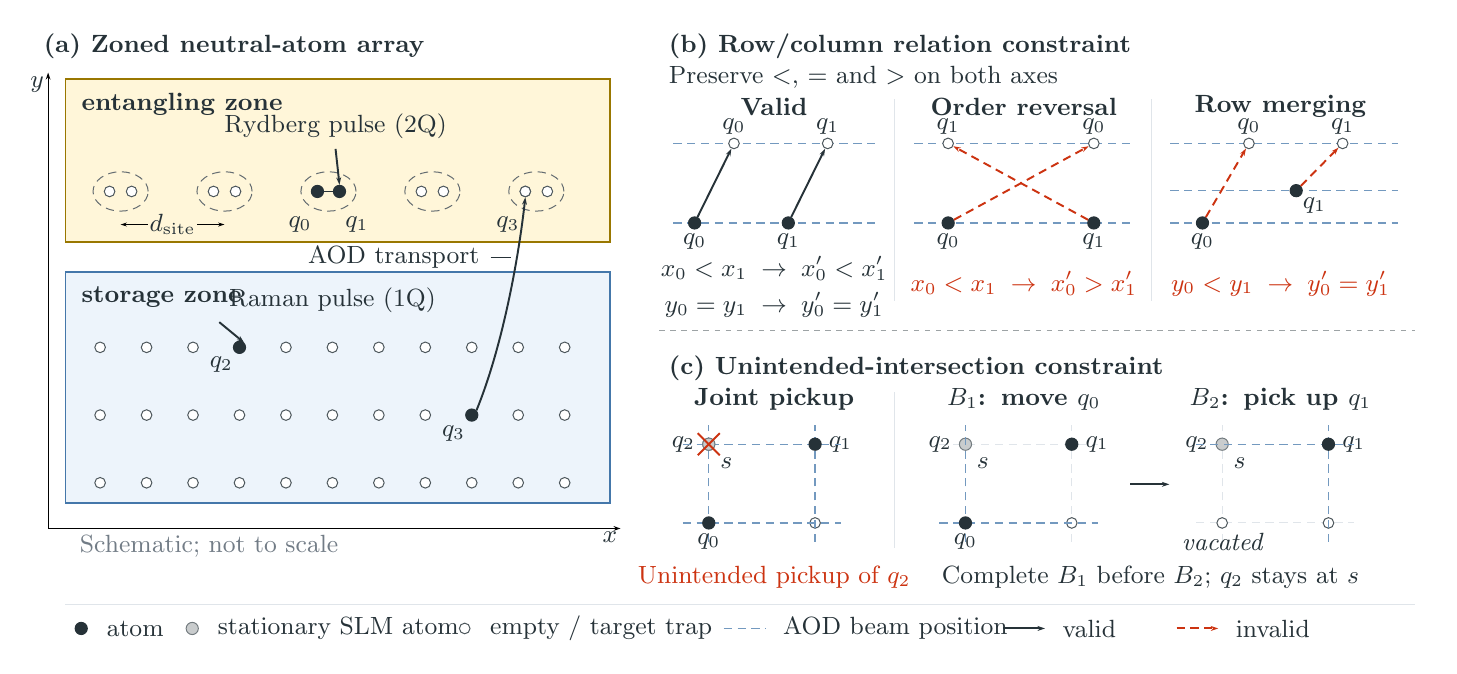
\begin{tikzpicture}[
  galk/base,x=1cm,y=1cm,
  trap/.style={galk/site},
  atom/.style={galk/occupied atom},
  fixed/.style={circle,draw=galkInk!65,line width=.35pt,fill=galkInk!25,
    minimum size=1.55mm,inner sep=0pt},
  motion/.style={galk/accepted path},
  guide/.style={draw=galkStorage!75,densely dashed,line width=.50pt},
  inactive guide/.style={draw=galkGrid,densely dashed,line width=.35pt},
  panel title/.style={galk/panel title},
  relation/.style={font=\rmfamily\fontsize{9.0pt}{10.0pt}\selectfont},
  case label/.style={font=\rmfamily\bfseries\fontsize{9.0pt}{10.0pt}\selectfont,
    text width=2.85cm,align=center,inner sep=1pt},
  explanatory note/.style={font=\rmfamily\fontsize{9.0pt}{10.0pt}\selectfont},
  legend label/.style={font=\rmfamily\fontsize{9.0pt}{10.0pt}\selectfont},
  galk/q label/.append style={font=\rmfamily\itshape\fontsize{9.0pt}{10.0pt}\selectfont},
  constraint divider/.style={draw=galkInk!45,dash pattern=on 2pt off 2pt,line width=.45pt}
]
  \path[use as bounding box] (0,-.65) rectangle (17.80,7.20);

  % Device abstraction: rectangular zones and regular trap arrays.
  \node[panel title] at (.08,6.97) {(a) Zoned neutral-atom array};
  \draw[galk/entanglement zone] (.48,4.48) rectangle (7.40,6.55);
  \draw[galk/storage zone] (.48,1.16) rectangle (7.40,4.10);
  \node[galk/zone label] at (.66,6.39) {entangling zone};
  \node[galk/zone label] at (.66,3.94) {storage zone};

  % Five equally spaced Rydberg sites, with two traps per site.
  \foreach \cx in {1.18,2.50,3.82,5.14,6.46} {
    \draw[galk/rydberg pair] (\cx,5.12) ellipse (.35 and .25);
    \node[trap] at (\cx-.14,5.12) {};
    \node[trap] at (\cx+.14,5.12) {};
  }
  \node[atom] (qzero) at (3.68,5.12) {};
  \node[atom] (qone) at (3.96,5.12) {};
  \draw[galkInk,line width=.48pt] (qzero)--(qone);
  \node[galk/q label,anchor=north east] at (3.62,4.81) {$q_0$};
  \node[galk/q label,anchor=north west] at (4.02,4.81) {$q_1$};
  \node[anchor=south] (rydberg) at (3.91,5.66) {Rydberg pulse (2Q)};
  \draw[motion] (rydberg.south)--(qone.north);

  % Three regular rows show the same occupied traps with fewer empty sites.
  \foreach \x in {.92,1.51,2.10,2.69,3.28,3.87,4.46,5.05,5.64,6.23,6.82} {
    \foreach \y in {1.42,2.28,3.14} {
      \node[trap] at (\x,\y) {};
    }
  }
  \node[atom] (qtwo) at (2.69,3.14) {};
  \node[galk/q label,anchor=north east] at (2.62,3.03) {$q_2$};
  \node[anchor=south] (raman) at (3.87,3.46) {Raman pulse (1Q)};
  \draw[motion] (raman.south west)--(qtwo.north east);

  % A hollow destination and one arrow denote a single transported atom.
  \node[atom] (qthree) at (5.64,2.28) {};
  \node[galk/q label,anchor=north east] at (5.57,2.16) {$q_3$};
  \node[trap] (qthreeDest) at (6.32,5.12) {};
  \draw[motion] (qthree.north east)
    .. controls (6.02,3.12) and (6.23,4.23) .. (qthreeDest.south);
  \node[galk/q label,anchor=north east] at (6.26,4.81) {$q_3$};
  \node[anchor=east] at (5.86,4.28) {AOD transport};
  \draw[galkInk,line width=.38pt] (5.88,4.28)--(6.14,4.28);

  \draw[-{Stealth[length=.9mm,width=.6mm]},line width=.42pt]
    (.26,.84)--(7.53,.84) node[below left,inner sep=1pt] {$x$};
  \draw[-{Stealth[length=.9mm,width=.6mm]},line width=.42pt]
    (.26,.84)--(.26,6.63);
  \node[anchor=center,inner sep=0pt] at (.12,6.48) {$y$};
  \draw[{Stealth[length=.8mm,width=.5mm]}-{Stealth[length=.8mm,width=.5mm]},
    line width=.38pt] (1.18,4.70)--(2.50,4.70);
  \node[fill=galkEntangleFill,inner sep=.7pt] at (1.84,4.70) {$d_{\rm site}$};
  \node[anchor=west,text=galkMuted,explanatory note]
    at (.54,.62) {Schematic; not to scale};

  % Strict ordering and row/column membership are one relation constraint.
  \node[panel title] at (8.02,6.97) {(b) Row/column relation constraint};
  \node[anchor=west] at (8.02,6.57) {Preserve $<$, $=$ and $>$ on both axes};
  \node[case label] at (9.48,6.20) {Valid};
  \node[case label] at (12.65,6.20) {Order reversal};
  \node[case label] at (15.91,6.20) {Row merging};
  \draw[galkGrid,line width=.38pt] (11.01,3.73)--(11.01,6.30);
  \draw[galkGrid,line width=.38pt] (14.27,3.73)--(14.27,6.30);

  % Valid: the common row and the order of two columns are preserved.
  \draw[guide] (8.20,4.72)--(10.79,4.72);
  \draw[guide] (8.20,5.73)--(10.79,5.73);
  \node[atom] (v0s) at (8.47,4.72) {};
  \node[atom] (v1s) at (9.66,4.72) {};
  \node[trap] (v0t) at (8.97,5.73) {};
  \node[trap] (v1t) at (10.16,5.73) {};
  \draw[motion] (v0s)--(v0t);
  \draw[motion] (v1s)--(v1t);
  \node[galk/q label,anchor=north] at (8.47,4.60) {$q_0$};
  \node[galk/q label,anchor=north] at (9.66,4.60) {$q_1$};
  \node[galk/q label,anchor=south] at (8.97,5.83) {$q_0$};
  \node[galk/q label,anchor=south] at (10.16,5.83) {$q_1$};
  \node[relation] at (9.48,4.14) {$x_0<x_1\;\to\;x'_0<x'_1$};
  \node[relation] at (9.48,3.68) {$y_0=y_1\;\to\;y'_0=y'_1$};

  % Invalid: column order reverses, while the common row remains unchanged.
  \draw[guide] (11.26,4.72)--(14.00,4.72);
  \draw[guide] (11.26,5.73)--(14.00,5.73);
  \node[atom] (o0s) at (11.69,4.72) {};
  \node[atom] (o1s) at (13.54,4.72) {};
  \node[trap] (o0t) at (13.54,5.73) {};
  \node[trap] (o1t) at (11.69,5.73) {};
  \draw[galk/invalid path] (o0s)--(o0t);
  \draw[galk/invalid path] (o1s)--(o1t);
  \node[galk/q label,anchor=north] at (11.69,4.60) {$q_0$};
  \node[galk/q label,anchor=north] at (13.54,4.60) {$q_1$};
  \node[galk/q label,anchor=south] at (13.54,5.83) {$q_0$};
  \node[galk/q label,anchor=south] at (11.69,5.83) {$q_1$};
  \node[relation,text=galkBad] at (12.65,3.95)
    {$x_0<x_1\;\to\;x'_0>x'_1$};

  % Invalid without a geometric crossing: distinct source rows merge.
  \draw[guide] (14.51,4.72)--(17.40,4.72);
  \draw[guide] (14.51,5.13)--(17.40,5.13);
  \draw[guide] (14.51,5.73)--(17.40,5.73);
  \node[atom] (m0s) at (14.92,4.72) {};
  \node[atom] (m1s) at (16.11,5.13) {};
  \node[trap] (m0t) at (15.51,5.73) {};
  \node[trap] (m1t) at (16.70,5.73) {};
  \draw[galk/invalid path] (m0s)--(m0t);
  \draw[galk/invalid path] (m1s)--(m1t);
  \node[galk/q label,anchor=north] at (14.92,4.60) {$q_0$};
  \node[galk/q label,anchor=north west] at (16.18,5.05) {$q_1$};
  \node[galk/q label,anchor=south] at (15.51,5.83) {$q_0$};
  \node[galk/q label,anchor=south] at (16.70,5.83) {$q_1$};
  \node[relation,text=galkBad] at (15.91,3.95)
    {$y_0<y_1\;\to\;y'_0=y'_1$};

  % Separate the two constraint classes without reducing the diagrams or text.
  \draw[constraint divider] (8.02,3.35)--(17.62,3.35);

  % The second constraint is the Cartesian product of activated beams.
  \begin{scope}[yshift=-.45cm]
  \node[panel title] at (8.02,3.33) {(c) Unintended-intersection constraint};
  \node[case label] at (9.48,2.93) {Joint pickup};
  \node[case label] at (12.65,2.93) {$B_1$: move $q_0$};
  \node[case label] at (15.91,2.93) {$B_2$: pick up $q_1$};
  \draw[galkGrid,line width=.38pt] (11.01,1.04)--(11.01,3.02);

  % Identical coordinates; the same stationary atom q2 is shown each time.
  \foreach \dx in {0,3.26,6.52} {
    \begin{scope}[xshift=\dx cm]
      \foreach \x in {8.65,10.00} {
        \draw[inactive guide] (\x,1.12)--(\x,2.61);
      }
      \foreach \y in {1.36,2.36} {
        \draw[inactive guide] (8.32,\y)--(10.33,\y);
      }
      \node[trap] at (10.00,1.36) {};
      \node[fixed] at (8.65,2.36) {};
      \node[galk/q label,anchor=east] at (8.49,2.36) {$q_2$};
      \node[galk/q label,anchor=north west] at (8.78,2.20) {$s$};
      \node[galk/q label,anchor=west] at (10.16,2.36) {$q_1$};
    \end{scope}
  }

  % Two rows and two columns also activate the occupied cross-intersection.
  \foreach \x in {8.65,10.00} {
    \draw[guide] (\x,1.12)--(\x,2.61);
  }
  \foreach \y in {1.36,2.36} {
    \draw[guide] (8.32,\y)--(10.33,\y);
  }
  \node[atom] at (8.65,1.36) {};
  \node[atom] at (10.00,2.36) {};
  \node[fixed] at (8.65,2.36) {};
  \node[galk/q label,anchor=north] at (8.65,1.24) {$q_0$};
  \draw[galkBad,line width=.7pt] (8.51,2.22)--(8.79,2.50);
  \draw[galkBad,line width=.7pt] (8.51,2.50)--(8.79,2.22);
  \node[explanatory note,text=galkBad,anchor=center]
    at (9.48,.67) {Unintended pickup of $q_2$};

  % Each snapshot shows only the pickup end of a complete serialized batch.
  % B1 transports and unloads q0 outside this view, then switches its beams off.
  \draw[guide] (11.91,1.12)--(11.91,2.61);
  \draw[guide] (11.58,1.36)--(13.59,1.36);
  \node[atom] at (11.91,1.36) {};
  \node[atom] at (13.26,2.36) {};
  \node[galk/q label,anchor=north] at (11.91,1.24) {$q_0$};
  \draw[motion] (14.00,1.85)--(14.50,1.85);
  \draw[guide] (16.52,1.12)--(16.52,2.61);
  \draw[guide] (14.84,2.36)--(16.85,2.36);
  \node[trap] at (15.17,1.36) {};
  \node[atom] at (16.52,2.36) {};
  \node[galk/q label,anchor=north] at (15.17,1.24) {vacated};
  \node[explanatory note,anchor=center] at (14.26,.67)
    {Complete $B_1$ before $B_2$; $q_2$ stays at $s$};
  \end{scope}

  % A dedicated legend row does not obscure any physical component.
  \begin{scope}[yshift=-.45cm]
  \draw[galkGrid,line width=.38pt] (.48,.32)--(17.62,.32);
  \node[atom] at (.68,.02) {};
  \node[anchor=west,legend label] at (.88,.02) {atom};
  \node[fixed] at (2.09,.02) {};
  \node[anchor=west,legend label] at (2.29,.02) {stationary SLM atom};
  \node[trap] at (5.55,.02) {};
  \node[anchor=west,legend label] at (5.75,.02) {empty / target trap};
  \draw[guide] (8.84,.02)--(9.37,.02);
  \node[anchor=west,legend label] at (9.47,.02) {AOD beam position};
  \draw[motion] (12.39,.02)--(12.92,.02);
  \node[anchor=west,legend label] at (13.02,.02) {valid};
  \draw[galk/invalid path] (14.59,.02)--(15.12,.02);
  \node[anchor=west,legend label] at (15.22,.02) {invalid};
  \end{scope}
\end{tikzpicture}
}
  \caption{分区架构与AOD约束。(a) $q_0$、$q_1$执行CZ门，$q_2$接受单比特旋转，$q_3$跨区输运；$d_{\rm site}$为相邻门位对的中心间距。(b) 行列次序与合并约束。(c) 联合拾取会误触静止于$s$的$q_2$；$B_1$先运走并卸载$q_0$，关闭该批行列后，$B_2$再拾取$q_1$。仅画拾取端，区域与阱数为示意。}
  \label{fig:architecture-preliminaries}
\end{figure*}

\subsection{分区架构与物理代价}
\label{sec:background}

空间光调制器（SLM）在存储区和纠缠区形成静态阱，声光偏转器（AOD）形成行列可调的移动阱。原子经SLM到AOD的转移、输运和AOD到SLM的转移到达目标位置，见图~\ref{fig:architecture-preliminaries}(a)。存储区与Rydberg照射区域隔离，纠缠区则采用成对阱位，使目标原子在全局Rydberg脉冲下执行CZ门；单比特旋转由可寻址Raman光束执行\cite{evered2023highfidelity,lin2025zac}。纠缠区非参与原子也会受激，因此驻留需要权衡转移与受激损失。

同批AOD输运须满足两类约束\cite{stade2024abstractmodel,stade2025routingaware}。首先，活动行列保持次序及同行同列关系。对源坐标$(x_i,y_i)$、$(x_j,y_j)$与目标坐标$(x'_i,y'_i)$、$(x'_j,y'_j)$，任意\mbox{$\star\in\{<,=,>\}$}均须满足
\begin{equation}
\begin{aligned}
x_i\star x_j&\ \Longleftrightarrow\ x'_i\star x'_j,\\
y_i\star y_j&\ \Longleftrightarrow\ y'_i\star y'_j.
\end{aligned}
\label{eq:aod-relations}
\end{equation}
因此，不相交的路径也可能无法并行，见图~\ref{fig:architecture-preliminaries}(b)。其次，活动行列在所有交点形成光阱，未承载目标原子的交点称为非目标交点（ghost spot）。在本文的执行模型中，拾取、输运和放下过程中，移动阱及非目标交点均不得扫过静止原子；这一检查也适用于单条轨迹。图~\ref{fig:architecture-preliminaries}(c)通过分批避免误拾取。目标阱还须满足占位依赖：原子转入AOD时即释放源SLM阱\cite{lin2025zac}，静止原子的阱位则不能通过交换批次次序释放。

放置由此影响阱转移、空闲受激以及分批输运中的相干时间消耗。为在同一尺度上比较这些代价，执行质量采用分区架构的保真度模型\cite{lin2025zac}：
\begin{equation}
\begin{aligned}
\log F={}&N_1\log f_1+N_2\log f_2
+N_{\mathrm{exc}}\log f_{\mathrm{exc}}\\
&+N_{\mathrm{tran}}\log f_{\mathrm{tran}}
+\sum_{q\in\mathcal Q}\log\left(1-\frac{t_q}{T_2}\right).
\end{aligned}
\label{eq:fidelity}
\end{equation}
其中，$N_1$、$N_2$为单、双比特门数，$N_{\mathrm{exc}}$为空闲受激次数，$N_{\mathrm{tran}}$为逐原子SLM/AOD阱转移次数，$f_1$、$f_2$、$f_{\mathrm{exc}}$、$f_{\mathrm{tran}}$为对应的单次保真度因子；$t_q$为原子$q\in\mathcal Q$的累计空闲时间，$T_2$为相干时间。门序列固定后，放置通过后三项影响保真度。相容轨迹构成重排批次，各批顺序执行。单个并行移动阶段的时长由最长轨迹决定\cite{stade2025routingaware}，完整批次还包含阱转移\cite{lin2025zac}。

\begin{samepage}
仅计转移与受激时，跨过$r$个空闲门层的驻留损失为$-r\log f_{\rm exc}$，往返为$-4\log f_{\rm tran}$。在$f_{\rm exc}=\ArgumentExcitationFidelity$、$f_{\rm tran}=\ArgumentTransferFidelity$时，$r=1$时驻留损失较低，$r=2$时往返损失较低。即使在这一双因子算例中，下次交互相隔的门层数也会改变当前选择；实际放置还须考虑占位、路由与相干影响。\par
\end{samepage}

\subsection{放置挑战与相关编译方法}

为降低交互带来的移动代价，已有中性原子编译方法优化原生门分解、交互感知布局和原子移动路由\cite{patel2022geyser,patel2023graphine,tan2022mapping,schmid2024hybrid}，并协调门调度与原子移动\cite{tan2024olsqdpqa,tan2025enola}。多阵列并行输运\cite{wang2024atomique}、免SWAP移动\cite{ludmir2024parallax}、移动辅助原子\cite{wang2024qpilot}及可重定向编译\cite{kirmemis2025weaver}进一步拓展了移动与交互的实现方式。面向分区执行，PowerMove协调门层调度与布局转换\cite{ruan2025powermove}，Mantra则通过程序改写减少输运\cite{jang2025mantra}。

在具体的放置决策中，ZAC通过相邻层匹配复用原子，并将后续伙伴距离计入门位和存储位匹配\cite{lin2025zac}。路由感知放置用A*选择门位和中间位置，评价移动相容性、批次时延、后续伙伴距离及复用节省的转移\cite{stade2025routingaware}。ZAP比较下次使用前的受激损失与回迁的转移、退相干损失，再按距离和冲突数逐门选择位置\cite{huang2026zap}。

这些方法已考虑复用、未来交互或物理代价。这些因素相互关联：保留原子会限制可用门位，回迁则改变后续输运的起点\cite{lin2025zac}。比较完整联合方案，需要追踪各方案执行后的配置如何影响后续门层的物理损失。

\label{sec:contributions}
为此，本文提出结合遗传搜索与多层前瞻的联合放置编译器GA-LK。该编译器联合优化门位、原子驻留和回迁存储位，在共同的占位与输运约束下比较完整方案，允许原子跨过其不参与的门层继续驻留；并从各候选的执行后配置出发，预测后续多层物理损失。遗传搜索在统一尺度上比较当前与后续损失，据此选择当前层的方案。

% Queue the full framework before the method begins.
\begin{figure*}[t]
  \centering
  \providecommand{\PaperOverallFigurePath}{build/paper_zh/figures/overall_framework.pdf}
  \includegraphics[width=\textwidth]{\PaperOverallFigurePath}
  \caption{GA-LK编译框架。前两列展示重基后同一电路的依赖保持调度，双实心点表示CZ，$U_3$统一表示单比特门。中间展开一般门层$\ell$的联合优化：当前执行产生候选后配置，未来层继承该配置并形成预测评分。虚线表示预测及评分反馈，底部实线传递实际层间配置。}
  \label{fig:overall-framework}
\end{figure*}

\begin{samepage}
\section{方法}
\label{sec:method}
\label{sec:formulation}

GA-LK将当前层放置与它留下的后续执行起点一并考虑。如图~\ref{fig:overall-framework}所示，门位、驻留与回迁存储位组成完整候选，物理评价将其转化为执行批次，得到当前损失与执行后配置；多层前瞻从这一配置继续预测，遗传搜索据此比较联合方案。选定后仅执行当前层，将实际配置传入下一层优化，使预测始终衔接已执行的决策。
\par\end{samepage}

\begin{algorithm}[!t]
\caption{联合放置的遗传搜索与多层前瞻}
\label{alg:solver}
\PaperAlgorithmSetup
\algrenewcommand\algorithmicrequire{\textbf{输入：}}
\algrenewcommand\algorithmicensure{\textbf{输出：}}
\algrenewcommand\algorithmicwhile{\textbf{当}}
\algrenewcommand\algorithmicdo{\textbf{时}}
\algrenewcommand\algorithmicfor{\textbf{对}}
\algrenewcommand\algorithmicif{\textbf{若}}
\algrenewcommand\algorithmicthen{\textbf{则}}
\algrenewcommand\algorithmicelse{\textbf{否则}}
\algrenewcommand\algorithmicreturn{\textbf{返回}}
\begin{algorithmic}[1]
\Require 配置$\mathbf{s}_\ell$；本层及后续门序列
\Ensure 所选方案、当前层批次及$\mathbf{s}_{\ell+1}$
\PaperAlgorithmPhase{I}{联合搜索与跨层评价}
\State 构造种子编码；按空间大小选择枚举或GA
\While{仍有未评价编码且预算未耗尽}
  \State 为编码$\mathbf x_\ell$匹配至多$K$个存储位分配
  \For{每个完整候选$(\mathbf x_\ell,a_\ell)$}
    \State \textbf{当前执行：}生成批次，不可行则跳过 \label{alg:route}
    \State 由批次及门操作计算$C_\ell^{\rm cur}$与$\mathbf{s}_{\ell+1}$
    \State \textbf{多层前瞻：}从$\mathbf{s}_{\ell+1}$逐层预测损失
    \State 按式~\eqref{eq:lookahead-cost}合成$J_\ell$，记录预测可行性 \label{alg:predict}
  \EndFor
  \State 由完整候选评分确定适应度，缓存结果
  \State 交叉、变异并保留精英，或继续枚举
\EndWhile
\State 有限局部调整后，按第~\ref{alg:route}--\ref{alg:predict}行重新评价
\PaperAlgorithmPhase{II}{选择并推进当前层}
\State 按参照、准入及排序规则选择方案
\State 提交当前层批次与门操作，更新实际配置
\State \Return 方案、批次及实际配置$\mathbf{s}_{\ell+1}$
\end{algorithmic}
\end{algorithm}


\subsection{联合放置建模}

联合方案同时指定门在哪里执行、哪些原子驻留及其余原子的回迁位置。输入为逻辑电路、阱阵列、原生门和输运约束，输出为可执行ZAIR指令。

候选按固定门层比较。门调度沿用类似ZAC的尽早执行策略\cite{lin2025zac}，交替组织单、双比特层。双比特门进入前驱均已完成的最早层，同层不共享原子，可由一次全局Rydberg脉冲执行多个CZ门；超出门位容量时拆层，可交换次序的门按交互图边着色分组。单比特门在各自双比特前驱完成后执行，无此类前驱时置于首层之前。记第$\ell$个双比特层及其门集合为$L_\ell$、$\mathcal G_\ell$，层前配置$\mathbf{s}_\ell$包含原子位置、阱位占用与执行时序状态，后者记录各原子累计空闲时间及资源依赖时刻。本层及相应单比特门执行后得到$\mathbf{s}_{\ell+1}$。

\begin{samepage}
被非参与原子占据的门位须先腾空，保留该原子则须另选门位，因此门位与驻留联合编码为
\begin{equation}
\mathbf x_\ell=
(z_{\ell,1},\ldots,z_{\ell,m},
 b_{\ell,1},\ldots,b_{\ell,k}).
\label{eq:chromosome}
\end{equation}
\end{samepage}
前$m$个基因选择门位对及方向，后$k$个基因决定驻留，0为保留、1为回迁。驻留位通常对应本层非参与的纠缠区原子；单门层可另含区内参与原子，以比较区内换位与回迁后重新入区。

门位满足纠缠区几何与容量约束，一侧已有参与原子时可只移动另一原子，两者都需移动时共同选择门位对及方向。长电路中的稀疏门层先搜索两原子附近的门位，输运不可行时扩展至全部门位。

回迁存储位同时影响本次离区与下次入区，候选存储阱取自当前纠缠位、初始存储位附近；若下次双比特交互位于预测范围内，则补充另一参与原子当前位置附近的存储阱，该原子在纠缠区时以最近存储阱为中心。每个回迁原子最多保留六个位置，再按距离生成前$K$个最小权匹配$a_\ell$\cite{murty1968assignment}。每个匹配将回迁原子分配至互不重复的存储阱，与编码$\mathbf x_\ell$组成完整候选$(\mathbf x_\ell,a_\ell)$。距离缩小候选存储阱的范围，随后按物理执行损失比较完整方案。

编码$(T_1^+,T_2^+,1)$选择门对$(q_0,q_2)$、$(q_1,q_4)$，匹配将$q_3$分配至$s_1$，如图~\ref{fig:joint-ga}所示。这一目标配置不能直接实现：$q_1$与$q_2$互占目标阱，同时交换违反行列次序，逐个执行又受目标占位阻挡。批次$B_0$因此在回迁$q_3$的同时暂存$q_1$，再由$B_1$--$B_3$依次放置$q_2,q_1,q_4$，$q_0$不动。中转不增加驻留基因，其开销必须计入该候选的物理评价；执行后的配置则成为后续门层的起点。

\begin{figure}[!t]
  \centering
  \resizebox{\columnwidth}{!}{% Figure colours remain semantic in both review and clean manuscripts.
\begingroup
\PaperShowRevisionsfalse
% Shared vector-figure vocabulary for the Chinese IEEE manuscript.
% Every figure in this directory inputs this file, so the manuscript only
% needs the standard TikZ package and the libraries already loaded by
% paper_zh.tex.  Keep the guard: figures may be input more than once while
% editing or when a stand-alone smoke-test document is built.
\ifdefined\GALKFigureStyleLoaded\else
\def\GALKFigureStyleLoaded{1}

% Indigo / blue / ochre palette adapted from Paul Tol qualitative schemes.
% Source: https://sronpersonalpages.nl/~pault/ (accessed 2026-09-14).
% Dark strokes identify roles; pale fills preserve text contrast.
% Atoms are filled, traps hollow, predictions dashed, invalid paths crossed.
\definecolor{galkInk}{HTML}{263238}
\definecolor{galkMuted}{HTML}{727C86}
\definecolor{galkGrid}{HTML}{E0E5EA}
\definecolor{galkFrame}{HTML}{A4AFBA}
\definecolor{galkPaper}{HTML}{FFFFFF}
% Blue and ochre identify storage and entangling zones; indigo highlights GA-LK.
% Forecasts use magenta dashes; comparison series retain grey open markers.
\definecolor{galkStorage}{HTML}{4477AA}
\definecolor{galkStorageFill}{HTML}{EDF4FB}
\definecolor{galkEntangle}{HTML}{997700}
\definecolor{galkEntangleFill}{HTML}{FFF6D9}
\definecolor{galkResident}{HTML}{332288}
\definecolor{galkResidentFill}{HTML}{F0EFF8}
\definecolor{galkGood}{HTML}{263238}
\definecolor{galkBad}{HTML}{CC3311}
\definecolor{galkLook}{HTML}{AA3377}
\definecolor{galkLookFill}{HTML}{F7EDF3}
\definecolor{galkData}{HTML}{332288}
\definecolor{galkTail}{HTML}{929AA3}
\definecolor{galkZAC}{HTML}{727C86}
\definecolor{galkICCAD}{HTML}{929AA3}
\definecolor{galkGroupOne}{HTML}{332288}
\definecolor{galkGroupTwo}{HTML}{727C86}
\definecolor{galkGroupThree}{HTML}{929AA3}

\tikzset{
  % Shared engineering-figure contract.  Physical snapshots must place an
  % paired-trap entanglement band above a dense storage field; only their scale may
  % change.  Labels are aligned at the upper-left of both regions.
  galk/base/.style={
    font=\rmfamily\fontsize{9.0pt}{10.0pt}\selectfont,
    text=galkInk,
    line cap=butt,
    line join=miter,
    >=Stealth
  },
  galk/panel title/.style={
    font=\rmfamily\bfseries\fontsize{9.0pt}{10.0pt}\selectfont,
    text=galkInk,
    anchor=west
  },
  galk/label/.style={
    font=\rmfamily\fontsize{9.0pt}{10.0pt}\selectfont,
    text=galkInk
  },
  galk/small label/.style={
    font=\rmfamily\fontsize{8.7pt}{9.7pt}\selectfont,
    text=galkInk
  },
  galk/zone label/.style={
    font=\rmfamily\bfseries\fontsize{8.7pt}{9.7pt}\selectfont,
    text=galkInk,
    anchor=north west,
    inner sep=.5pt
  },
  galk/entanglement zone/.style={
    draw=galkEntangle,
    fill=galkEntangleFill,
    line width=.65pt
  },
  galk/storage zone/.style={
    draw=galkStorage,
    fill=galkStorageFill,
    line width=.65pt
  },
  galk/site/.style={
    circle,
    draw=galkInk!82,
    fill=white,
    line width=.36pt,
    minimum size=1.35mm,
    inner sep=0pt
  },
  galk/occupied atom/.style={
    circle,
    draw=galkInk,
    fill=galkInk,
    line width=.36pt,
    minimum size=1.55mm,
    inner sep=0pt
  },
  galk/target site/.style={
    circle,
    draw=galkInk!60,
    fill=galkInk!10,
    line width=.34pt,
    minimum size=1.55mm,
    inner sep=0pt
  },
  galk/q label/.style={
    font=\rmfamily\itshape\fontsize{8.5pt}{9.5pt}\selectfont,
    text=galkInk,
    inner sep=.25pt
  },
  galk/rydberg pair/.style={
    draw=galkInk!72,
    densely dashed,
    line width=.36pt
  },
  galk/accepted path/.style={
    -{Stealth[length=.95mm,width=.62mm]},
    draw=galkInk,
    line width=.70pt
  },
  galk/alternative path/.style={
    -{Stealth[length=.95mm,width=.62mm]},
    draw=galkMuted,
    densely dashed,
    line width=.65pt
  },
  galk/future path/.style={
    -{Stealth[length=.95mm,width=.62mm]},
    draw=galkLook,
    densely dashed,
    line width=.70pt
  },
  galk/invalid path/.style={
    -{Stealth[length=.95mm,width=.62mm]},
    draw=galkBad,
    densely dashed,
    line width=.70pt
  }
}
\fi

\providecommand{\PaperRevision}[1]{#1}
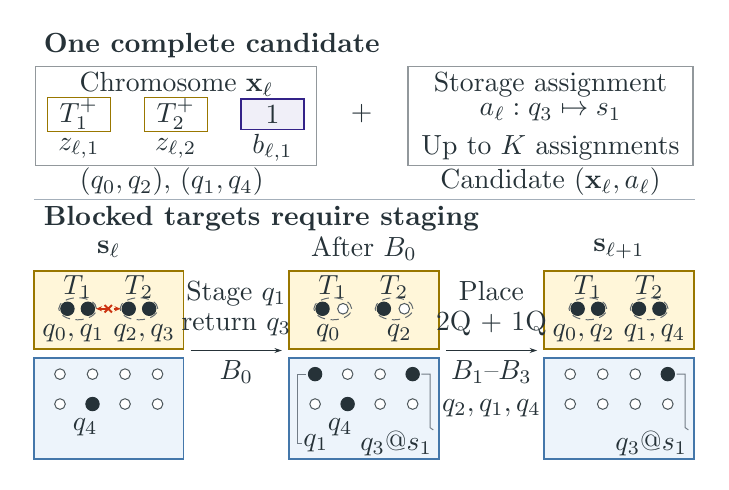
\begin{tikzpicture}[
  galk/base,x=1cm,y=1cm,
  panel title/.style={galk/panel title,font=\rmfamily\bfseries\fontsize{10pt}{11pt}\selectfont},
  label/.style={font=\rmfamily\fontsize{10pt}{11pt}\selectfont},
  note/.style={font=\rmfamily\fontsize{10pt}{11pt}\selectfont},
  rule/.style={draw=galkFrame,line width=.50pt},
  flow/.style={galk/accepted path},
  cell/.style={draw=galkInk!72,fill=white,line width=.50pt,
    minimum width=.80cm,minimum height=.39cm,inner sep=.5pt,
    font=\rmfamily\fontsize{10pt}{11pt}\selectfont},
  gate cell/.style={cell,draw=galkEntangle},
  bit cell/.style={cell,draw=galkResident,fill=galkResidentFill},
  gene/.style={minimum width=.54cm,minimum height=.33cm,inner sep=.4pt,
    font=\rmfamily\fontsize{10pt}{11pt}\selectfont},
  trap/.style={galk/site},
  atom/.style={galk/occupied atom,minimum size=1.7mm},
  q label/.style={galk/q label,font=\rmfamily\fontsize{10pt}{11pt}\selectfont}
]
  \path[use as bounding box] (0,2.43) rectangle (8.55,7.95);
  \node[panel title] at (.08,7.72)
    {\PaperRevision{One complete candidate}};
  \draw[draw=galkInk!50,line width=.45pt] (.10,6.20) rectangle (3.67,7.46);
  \draw[draw=galkInk!50,line width=.45pt] (4.83,6.20) rectangle (8.45,7.46);
  \node[label] at (1.89,7.23) {\PaperRevision{Chromosome $\mathbf{x}_\ell$}};
  \foreach \i/\head/\value/\cellstyle in {
    0/{$z_{\ell,1}$}/{$T_1^{+}$}/gate cell,
    1/{$z_{\ell,2}$}/{$T_2^{+}$}/gate cell,
    2/{$b_{\ell,1}$}/{1}/bit cell} {
    \node[\cellstyle] (gene-\i) at (.65+1.23*\i,6.85) {\PaperRevision{\value}};
    \node[note] at (.65+1.23*\i,6.42) {\PaperRevision{\head}};
  }
  \node[label] at (4.24,6.86) {\PaperRevision{$+$}};
  \node[label] at (6.64,7.23) {\PaperRevision{Storage assignment}};
  \node[label] at (6.64,6.87) {\PaperRevision{$a_\ell:q_3\mapsto s_1$}};
  \node[note] at (6.64,6.42) {\PaperRevision{Up to $K$ assignments}};
  \node[note] at (1.83,5.99)
    {\PaperRevision{$(q_0,q_2)$, $(q_1,q_4)$}};
  \node[label] at (6.64,5.99)
    {\PaperRevision{Candidate $(\mathbf{x}_\ell,a_\ell)$}};
  \draw[rule] (.08,5.77)--(8.47,5.77);

  % (b) The same regular array is used in all three snapshots. All five atoms
  % occur exactly once. s1 is the rightmost trap of the upper storage row.
  \node[panel title] at (.08,5.53)
    {\PaperRevision{Blocked targets require staging}};
  \def\routeInitial{0/.36/1.91,1/.58/1.91,2/1.02/1.91,3/1.24/1.91,4/.63/.70}
  \def\routeStaged{0/.36/1.91,1/.28/1.08,2/1.02/1.91,3/1.33/1.08,4/.63/.70}
  \def\routeFinal{0/.36/1.91,1/1.02/1.91,2/.58/1.91,3/1.33/1.08,4/1.24/1.91}
  % batch / atom / source x,y / target x,y; B0 temporarily stages q1.
  \def\routeMoves{0/1/.58/1.91/.28/1.08,0/3/1.24/1.91/1.33/1.08,1/2/1.02/1.91/.58/1.91,2/1/.28/1.08/1.02/1.91,3/4/.63/.70/1.24/1.91}
  \begin{scope}[yshift=2.47cm]
    \foreach \left in {.08,3.32,6.56} {
      \path[galk/entanglement zone] (\left,1.40) rectangle (\left+1.90,2.39);
      \path[galk/storage zone] (\left,0) rectangle (\left+1.90,1.28);
      \node[note] at (\left+.5546,2.19) {\PaperRevision{$T_1$}};
      \node[note] at (\left+1.3334,2.19) {\PaperRevision{$T_2$}};
      \draw[galk/rydberg pair] (\left+.5546,1.91) ellipse (.24 and .14);
      \draw[galk/rydberg pair] (\left+1.3334,1.91) ellipse (.24 and .14);
      \foreach \dx in {.36,.58,1.02,1.24}
        \node[trap] at (\left+1.18*\dx,1.91) {};
      \foreach \dx in {.28,.63,.98,1.33}
        \foreach \yy in {.70,1.08}
          \node[trap] at (\left+1.18*\dx,\yy) {};
    }
    \node[label] at (1.03,2.67) {\PaperRevision{$\mathbf{s}_\ell$}};
    \node[label] at (4.27,2.67) {\PaperRevision{After $B_0$}};
    \node[label] at (7.51,2.67) {\PaperRevision{$\mathbf{s}_{\ell+1}$}};
    \foreach \qq/\xx/\yy in \routeInitial
      \node[atom] at (.08+1.18*\xx,\yy) {};
    \foreach \qq/\xx/\yy in \routeStaged
      \node[atom] at (3.32+1.18*\xx,\yy) {};
    \foreach \qq/\xx/\yy in \routeFinal
      \node[atom] at (6.56+1.18*\xx,\yy) {};
    % Rejected endpoint-swap intention, not an executed AOD trajectory.
    % q1 and q2 occupy one another's chosen target traps before B0.
    \draw[draw=galkBad,densely dashed,line width=.60pt,
      {Stealth[length=.75mm,width=.65mm]}-{Stealth[length=.75mm,width=.65mm]},
      shorten <=1.05mm,shorten >=1.05mm]
      (.08+1.18*.58,1.91)--(.08+1.18*1.02,1.91);
    \draw[draw=galkBad,line width=.70pt]
      (1.024-.047,1.91-.047)--(1.024+.047,1.91+.047)
      (1.024-.047,1.91+.047)--(1.024+.047,1.91-.047);
    \foreach \xx/\lab in {.58/{$q_0,q_1$},1.48/{$q_2,q_3$},3.82/{$q_0$},4.72/{$q_2$},7.06/{$q_0,q_2$},7.96/{$q_1,q_4$}}
      \node[q label] at (\xx,1.60) {\PaperRevision{\lab}};
    \foreach \xx in {.73,3.97}
      \node[q label,anchor=north] at (\xx,.53) {\PaperRevision{$q_4$}};
    % Unarrowed leaders identify storage atoms without crossing any trap.
    % The lower storage margin is reserved for q1 and q3 labels.
    \node[q label] (stagedQOneLabel) at (3.66,.20) {\PaperRevision{$q_1$}};
    \draw[galkMuted,line width=.35pt]
      (3.54,1.08)--(3.43,1.08)--(3.43,.20)--(stagedQOneLabel.west);
    \foreach \i/\left in {1/3.32,2/6.56} {
      \node[q label] (storedQThreeLabel-\i) at (\left+1.36,.20)
        {\PaperRevision{$q_3@s_1$}};
      \draw[galkMuted,line width=.35pt]
        (\left+1.68,1.08)--(\left+1.79,1.08)--(\left+1.79,.40)
        --(storedQThreeLabel-\i.north east);
    }
    \draw[flow] (2.07,1.38)--(3.23,1.38);
    \node[note,align=center] at (2.65,1.91) {\PaperRevision{Stage $q_1$}\\\PaperRevision{return $q_3$}};
    \node[label] at (2.65,1.11) {\PaperRevision{$B_0$}};
    \draw[flow] (5.31,1.38)--(6.47,1.38);
    \node[note,align=center] at (5.89,1.91) {\PaperRevision{Place}\\\PaperRevision{2Q + 1Q}};
    \node[label] at (5.89,1.11) {\PaperRevision{$B_1$--$B_3$}};
    \node[note] at (5.89,.65) {\PaperRevision{$q_2,q_1,q_4$}};
  \end{scope}
\end{tikzpicture}
\endgroup
}
  \caption{完整候选从目标位置到可执行配置的转换。上方为编码与回迁分配，下方保持同一阵列与五个原子，展示目标受阻、中转及作为下一层起点的执行后配置。正负上标表示门位方向，从左至右为正；红色虚线为不可执行的交换意向。$s_1$为右侧存储阱，$B_0$--$B_3$为实际重排批次。}
  \label{fig:joint-ga}
\end{figure}

\subsection{跨层物理损失评价}

完整候选确定后，评价先生成其当前层执行批次：将回迁及阻挡目标门的原子移至存储区，再安排参与原子入区或区内换位，并随批次更新占位。依据式~\eqref{eq:fidelity}，省略固定门保真度项后，这些批次及门操作引起的新增负对数保真度损失为
\begin{equation}
\begin{aligned}
C_\ell^{\rm cur}={}&-\Delta N_{\rm tran}\log f_{\rm tran}
-\Delta N_{\rm exc}\log f_{\rm exc}\\
&+\sum_{q\in\mathcal Q}
\log\frac{1-t_q^{-}/T_2}{1-t_q^{+}/T_2},
\end{aligned}
\label{eq:current-cost}
\end{equation}
其中$\Delta N_{\rm tran}$、$\Delta N_{\rm exc}$为新增次数，$t_q^{-}$、$t_q^{+}$为批次和门依赖确定的执行前后累计空闲时间，$\mathcal Q$为原子集合。该可变损失增量由执行前后的累计值作差得到，后续每个预测层也采用同一计算方式。


前瞻进一步比较各候选留下的起点：从各自的$\mathbf{s}_{\ell+1}$出发，逐层更新位置、占位和时间。预测器按两参与原子的输运距离及阻挡原子的回迁距离贪心选择门位，使用本层尚未分配的合法门位并按固定次序破同分。受阻时先迁移阻挡原子，联合入区不可行时依次尝试有限中转和逐原子入区。每层的新增损失$\widehat C_{\ell,d}$由预测批次计算，后续层继承该层执行后的配置。

实际预测深度$h_\ell$满足$0\le h_\ell\le H$，$H$为后续双比特层数上限，$d=1$表示首个未来层。当前损失和衰减后的未来损失共同组成
\begin{equation}
J_\ell=C_\ell^{\rm cur}
+\sum_{d=1}^{h_\ell}\alpha\rho^{d-1}\widehat C_{\ell,d}
+\alpha\rho^{h_\ell-1}\Phi_\ell .
\label{eq:lookahead-cost}
\end{equation}
$\alpha$为未来损失权重，$\rho$为衰减系数。末端项$\Phi_\ell$估计最后一个预测层后仍在纠缠区、但未参与该层门操作的原子的可行回迁损失。预测在后续层用尽、达到规模相关的层数预算或$\rho^{d-1}<\epsilon$时截止；$H=0$或没有后续层时，$h_\ell=0$且未来层与末端项均取零。

\subsection{遗传搜索与初始布局}
\label{sec:initial-placement}

小规模联合空间直接枚举，超过阈值时采用GA\cite{holland1975adaptation}，以全驻留、全回迁和物理贪心方案为种子。交叉组合父代门位段与驻留段，变异修改门位、驻留位或冲突变量。解码将重复门位改至空闲门位，再匹配存储位并评价。

编码适应度取执行与预测均可行分配的最小$J_\ell$，并与同分规则共同决定个体保留。编码缓存避免重复评价，评价数或代数达到上限时停止。搜索结束后，先对候选作有限局部调整并重新评价，再确定参照并执行准入与排序，如算法~\ref{alg:solver}所示。单层搜索预算、$K$和前瞻范围随电路规模收缩。

未来门位来自近似预测，准入规则限制为预测收益增加的当前损失。在容量与强制回迁条件允许时，比较驻留至预测范围内的下次复用与往返存储区的损失，形成驻留建议。在执行与预测均可行的候选中，保留违反这些建议最少的一组，以该组当前损失最小者为参照，准入与排序仅在同组内进行；$H=0$时不启用驻留优先。

相对参照，若候选增加当前损失，增加量须不超过加权未来节省的四分之一，且$J_\ell$不升；未来节省含式~\eqref{eq:lookahead-cost}的未来层及末端项。通过者按$J_\ell$排序，再依次以批次数、重排时延、距离和固定编码次序破同分；没有更优者保留参照。当前不可执行的候选不参与选择；预测不可行则仅表示前瞻未找到后续路径，所有未来预测均不可行时按当前可执行代价选择，不存在当前可执行候选时报告失败。


执行开始前，初始布局已决定早期门层的输运起点。GA-LK因此沿用上述物理评价，以早期执行损失选择映射。存储阱按阵列次序，从最靠近纠缠区的一行起逐列选取，数量等于原子数；染色体按原子编号记录阱位索引，形成固定阱集合上的排列。

给定映射$\pi$，首层通过门位匹配及可行性修复生成方案；后续层调用联合优化，但关闭内层前瞻以限制每次映射评价的开销。评价轨迹仅在临时配置上更新路由、门执行、位置与时间。以$d=0$表示首个双比特层，之后实际评价$h_{\rm init}$层，目标为
\begin{equation}
J_{\rm init}(\pi)=
\sum_{d=0}^{h_{\rm init}}\rho^d\,\Delta C_d(\pi),
\qquad 0\le h_{\rm init}\le H_{\rm init}.
\label{eq:initial-lookahead}
\end{equation}
$\Delta C_d$为逐层新增负对数保真度损失，包含依赖要求的单比特门及其时间。$H_{\rm init}$限制后续层数；评价在门层完成后截止，仅到达真实末层时计入末端回迁，$H_{\rm init}=0$仍搜索首层损失。

初始化种群由顺序布局、按首次双比特交互排序及按加权交互强度排列的三个种子与扰动组成；种子可读取全电路交互，适应度仅评价早期前缀。锦标赛选择、顺序交叉（OX）和交换、插入、反转变异生成后代并保留精英。重复映射不再评价，唯一映射评价数、候选生成数、代数或停滞达到上限时停止。仅将$J_{\rm init}$最小的可行映射交给动态编译，无可行映射则报告失败。外层映射和内层编码分别设置预算，参数见第~\ref{sec:experimental-setup}节。

\subsection{物理约束下的编译输出}
\label{sec:routing}

为使前述损失对应可执行操作，候选评价与最终指令共用路由和时序规则。相容移动分组与阱位依赖分别承接路由感知放置和ZAC\cite{stade2025routingaware,lin2025zac}。冲突图以轨迹为顶点，将违反行列关系、或联合光阱在拾取、输运、释放时覆盖静止原子的轨迹相连。DSATUR着色\cite{brelaz1979coloring}分组后检查源阱释放、目标占用和AOD容量，不满足整体约束时拆批；单条轨迹扫过静止原子时迁移阻挡者、改道或否决候选。调度遵守原子、SLM、AOD和Rydberg依赖，源阱释放后才可复用。各批顺序执行，完整重排时延为
\begin{equation}
T_\ell^{\rm rr}=\sum_{b=1}^{B_\ell}T_{\ell,b}^{\rm batch},
\label{eq:rearrangement-metrics}
\end{equation}
式中$B_\ell$为批次数，$T_{\ell,b}^{\rm batch}$为第$b$批拾取、输运、释放及必要内部移动的总时长；这些执行时间参与相干损失计算。

所选方案的批次与门依赖写入ZAIR可执行序列\cite{lin2025zac}。重排指令记录原子起止位置和AOD操作，门指令采用执行时的原子映射，可寻址存储区或纠缠区，资源依赖和开始时刻共同确定顺序。末端回迁后，编译器验证完整序列的门操作、占位和AOD约束，并从中统计模型保真度、批次和时延。

\section{实验评估}
\label{sec:evaluation}

\subsection{比较设置}
\label{sec:experimental-setup}

实验将GA-LK与ZAC\cite{lin2025zac}及Stade等的路由感知放置\cite{stade2025routingaware}进行比较，基线采用其公开实现。\footnote{ZAC采用ASAP调度、动态放置与原子复用。路由感知基线采用MQT QMAP 3.2.0/Core 3.1.0，前瞻因子为0.2，深化值为0.2，复用级别为5，深化因子为0.6。}输入包括ZAC的18个基准电路（ZAC18）\cite{lin2025zac}与MQT QMAP示例集的154个输入文件\cite{wille2023qmap}，后者包含151个规范化后的不同电路，等价输入在聚合时合并。三种编译器接收相同门序列。基线沿用原始输出及既定验收口径，不追加修复或诊断筛选；GA-LK在候选评价中检查非目标交点与静止原子的冲突。

统一架构包含一个AOD、$100\times100$个存储阱和两块配对的$7\times20$纠缠阵列，共提供140个门位。式~\eqref{eq:fidelity}取$(f_1,f_2,f_{\rm tran},f_{\rm exc})=(0.9997,0.995,0.999,0.9975)$及$T_2=1.5$\,s，单比特门、CZ门和阱转移分别耗时52、0.36和15\,$\mu$s。质量比较纳入各参与配置均完成编译、且各原子空闲时间低于$T_2$的电路；主实验要求GA-LK三个种子均有效，逐电路取中位数。电路间保真度采用几何均值，批次和重排时延采用算术均值。

主比较采用各编译器自身的初始化。GA-LK初始化使用种群8、映射评价上限32，评价首层及后两层；初始化前缀内的后续层编码评价上限为32、内层前瞻关闭。动态优化取$H=8$、$\alpha=0.5$、$\rho=0.7$和$\epsilon=0.05$，编码评价上限576并按规模收缩。前瞻、搜索及预算对照固定起始映射，初始化对照则固定后续动态配置；各项研究按其参与配置分别确定样本。

\subsection{总体收益与物理来源}

GA-LK在两个电路集上相对两种基线均提高了保真度几何均值，并减少平均重排批次，如表~\ref{tab:main-results}所示。相对ZAC，ZAC18与QMAP的保真度分别提高\GAMainZACVsZACFidelityGain\%和\GAMainQMAPVsZACFidelityGain\%，QMAP的批次减少\GAMainQMAPVsZACBatchReduction\%。

\begin{table}[!tb]
\caption{\PaperRevision{两个电路集上三种编译方法的总体结果}}
\label{tab:main-results}
\centering
\PaperTableSetup
\fontsize{8.5pt}{9.7pt}\selectfont
\setlength{\tabcolsep}{1.2pt}
\begin{tabular*}{\columnwidth}{@{\extracolsep{\fill}}llrrrr@{}}
\toprule
数据集 & 方法 & \PaperRevision{保真度} & \PaperRevision{批次} & \shortstack{\PaperRevision{重排时延}\\\PaperRevision{(ms)}} & \shortstack{\PaperRevision{完成编译}\\\PaperRevision{/输入}}\\
\midrule
\multirow{3}{*}{\shortstack{ZAC18\\\PaperRevision{$N=\GAMainZACStrictN$}}}
& ZAC & \PaperRevision{\pgfmathprintnumber[fixed,precision=4,zerofill]{\GAMainZACMOneF}} & \PaperRevision{\GAMainZACMOneB} & \PaperRevision{\GAMainZACMOneT} & \PaperRevision{\GAMainZACMOneV}\\
& Stade等 & \PaperRevision{\pgfmathprintnumber[fixed,precision=4,zerofill]{\GAMainZACMTwoF}} & \PaperRevision{\GAMainZACMTwoB} & \PaperRevision{\textbf{\GAMainZACMTwoT}} & \PaperRevision{\GAMainZACMTwoV}\\
& GA-LK & \PaperRevision{\textbf{\boldmath\pgfmathprintnumber[fixed,precision=4,zerofill]{\GAMainZACMFourF}}} & \PaperRevision{\textbf{\GAMainZACMFourB}} & \PaperRevision{\GAMainZACMFourT} & \PaperRevision{\GAMainZACMFourV}\\
\midrule
\multirow{3}{*}{\shortstack{\PaperRevision{QMAP}\\\PaperRevision{$N=\GAMainQMAPStrictN$}}}
& ZAC & \PaperRevision{\pgfmathprintnumber[fixed,precision=6,zerofill]{\GAMainQMAPMOneF}} & \PaperRevision{\GAMainQMAPMOneB} & \PaperRevision{\GAMainQMAPMOneT} & \PaperRevision{\GAMainQMAPMOneV}\\
& Stade等 & \PaperRevision{\pgfmathprintnumber[fixed,precision=6,zerofill]{\GAMainQMAPMTwoF}} & \PaperRevision{\GAMainQMAPMTwoB} & \PaperRevision{\GAMainQMAPMTwoT} & \PaperRevision{\GAMainQMAPMTwoV}\\
& GA-LK & \PaperRevision{\textbf{\boldmath\pgfmathprintnumber[fixed,precision=6,zerofill]{\GAMainQMAPMFourF}}} & \PaperRevision{\textbf{\GAMainQMAPMFourB}} & \PaperRevision{\textbf{\GAMainQMAPMFourT}} & \PaperRevision{\GAMainQMAPMFourV}\\
\bottomrule
\end{tabular*}
\PaperTableNote[\columnwidth]{\fontsize{8pt}{9.1pt}\selectfont\PaperRevision{注：$N$为纳入质量比较的不同电路数；保真度取几何均值，重排批次和时延取算术均值。QMAP电路集的\GAMainQMAPStrictFileN{}个文件合并为\GAMainQMAPStrictN{}个不同电路。最后一列统计全部输入文件的编译完成数，包含超出保真度模型适用域的结果。粗体为同一电路集内的最优值。}}
\end{table}


不同电路集呈现出不同的收益分布。相对ZAC，ZAC18有\GAMainZACVsZACWins 个电路改善、\GAMainZACVsZACLosses 个下降，QMAP则为\GAMainQMAPVsZACWins 胜、\GAMainQMAPVsZACLosses 负；相对路由感知基线，QMAP为\GAMainQMAPVsICCADWins 胜、\GAMainQMAPVsICCADLosses 负。因此，QMAP的总体提升主要体现为部分电路上幅度较大的改善，而非更多电路获胜。几何均值通过对数保真度比的平均反映这一关系。

在两个电路集相对两种基线的比较中，阱转移与退相干损失的降低均超过新增空闲受激损失。QFT-18中，相对ZAC的阱转移由\GAMainMechanismQFTBaseTransfers 次降至\GAMainMechanismQFTGATransfers 次；转移、受激、相干分量对$\Delta\ln F$贡献的种子中位数依次为\mbox{$(+\GAMainMechanismQFTTransferGainRounded,\,\GAMainMechanismQFTExcitationGainRounded,\,+\GAMainMechanismQFTCoherenceGainRounded)$}。该例的主要收益来自阱转移减少。

\subsection{前瞻与搜索的作用}
\label{sec:ablation}

在相同联合决策空间中，考虑后续门层有助于改善方案选择。在固定初始映射、联合变量、搜索预算和存储位候选域的对照中，将$H=0$改为$H=8$，\AblationHN 个电路的保真度几何均值提高\PaperPercentGain{\AblationHRatio}{1}。$H=8$配置考虑后续门层、末端回迁及近期复用的驻留安排，$H=0$仅按当前层损失选择。

另一项对照固定跨层目标，考察遗传搜索如何从联合候选中作出选择。对于超出枚举阈值的空间，遗传搜索与逐坐标贪心使用相同的$H=8$、物理约束、目标函数、评价预算和局部精修规则；遗传搜索使\AblationGAN 个电路的保真度几何均值提高\PaperPercentGain{\AblationGARatio}{1}。两项对照分别考察前瞻配置与同一联合空间内的搜索差异，来自不同样本，其增量不能相加。

\label{sec:horizon-evaluation}
前瞻的收益还取决于预测范围。在独立的范围研究中，所测电路的大部分平均改善在一层前瞻时已经获得。图~\ref{fig:experimental-summary}展示\HorizonExtCompleteN 个电路的完整轨迹：从$H=0$增至1时，保真度比的几何均值提高、批次比的几何均值降低，继续扩大上限的平均变化较小。$H=4$与8有4个电路的实际窗口相同，体现了剩余层数和规模预算对预测展开的限制。

\begin{figure}[!htb]
  \centering
  \resizebox{\columnwidth}{!}{% Two side-by-side plots at final single-column width, following the supplied template.
% All ten circuit medians and both geometric means retain the frozen H8 normalization.
\begingroup
\PaperShowRevisionsfalse
\input{figures/tikz_style}
\pgfplotstableread[col sep=space]{figures/data/horizon_trends.dat}\HorizonTrendData
\begin{tikzpicture}[galk/base,
  horizon label/.style={font=\rmfamily\fontsize{10pt}{11pt}\selectfont}]
  \path[use as bounding box] (0,0) rectangle (8.80,4.49);
  \node[horizon label,font=\rmfamily\bfseries\fontsize{10pt}{11pt}\selectfont]
    at (2.70,4.24) {Fidelity};
  \node[horizon label,font=\rmfamily\bfseries\fontsize{10pt}{11pt}\selectfont]
    at (6.73,4.24) {Batches};
  \pgfplotsset{horizon trend axis/.style={
    width=3.16cm,height=2.45cm,scale only axis,
    axis lines*=left,axis line style={draw=galkInk,line width=.65pt},
    tick style={draw=galkInk,line width=.45pt},tick align=outside,
    tick label style={font=\rmfamily\fontsize{10pt}{11pt}\selectfont},
    label style={font=\rmfamily\fontsize{10pt}{11pt}\selectfont},
    xmin=-.15,xmax=8.2,xtick={0,1,2,4,8},
    ymajorgrids=true,grid style={draw=galkMuted!28,line width=.35pt},
    scaled ticks=false,clip=true,
  }}
  \begin{axis}[horizon trend axis,
    at={(1.12cm,1.43cm)},anchor=south west,
    ylabel={Ratio to $H=8$},
    ylabel style={at={(axis description cs:-.27,.5)},anchor=south,inner sep=0pt},
    ymin=.18,ymax=1.055,ytick={.2,.4,.6,.8,1.0}]
    \addplot[draw=galkMuted!85,densely dashed,line width=.55pt,forget plot] coordinates {(0,1) (8,1)};
    \pgfplotsinvokeforeach{0,...,9}{
      \addplot[draw=galkMuted!70,line width=.65pt,mark=*,mark size=.95pt,
        mark options={draw=galkMuted!85,fill=white},forget plot]
        table[x=horizon,y=f#1]{\HorizonTrendData};
    }
    \addplot[draw=galkData,line width=1.3pt,mark=diamond*,mark size=2pt,
      mark options={draw=white,line width=.4pt,fill=galkData}]
      table[x=horizon,y=f_mean]{\HorizonTrendData};
  \end{axis}
  \begin{axis}[horizon trend axis,
    at={(5.15cm,1.43cm)},anchor=south west,
    ymin=.95,ymax=1.73,ytick={1.0,1.2,1.4,1.6}]
    \addplot[draw=galkMuted!85,densely dashed,line width=.55pt,forget plot] coordinates {(0,1) (8,1)};
    \pgfplotsinvokeforeach{0,...,9}{
      \addplot[draw=galkMuted!70,line width=.65pt,mark=*,mark size=.95pt,
        mark options={draw=galkMuted!85,fill=white},forget plot]
        table[x=horizon,y=b#1]{\HorizonTrendData};
    }
    \addplot[draw=galkData,line width=1.3pt,mark=diamond*,mark size=2pt,
      mark options={draw=white,line width=.4pt,fill=galkData}]
      table[x=horizon,y=b_mean]{\HorizonTrendData};
  \end{axis}
  \node[horizon label] at (4.65,.64) {Look-ahead upper bound $H$};
  \draw[draw=galkMuted!70,line width=.65pt] (.32,.20)--(.86,.20);
  \node[circle,draw=galkMuted!85,fill=white,inner sep=1pt] at (.59,.20) {};
  \node[horizon label,anchor=west] at (.96,.20) {Circuits ($N=10$)};
  \draw[draw=galkData,line width=1.3pt] (4.70,.20)--(5.24,.20);
  \node[diamond,draw=white,fill=galkData,inner sep=1.3pt] at (4.97,.20) {};
  \node[horizon label,anchor=west] at (5.34,.20) {Geometric mean};
\end{tikzpicture}
\endgroup
}
  \caption{前瞻上限对编译结果的影响。各电路先取\HorizonExtSeedN 个种子的中位数，再以各自$H=8$的结果归一化。左右绘图区分别为保真度比和批次比；细线保留全部电路，粗线为\HorizonExtCompleteN 个电路的几何均值。$H$为上限，实际深度还受剩余层数与规模预算约束。}
  \label{fig:experimental-summary}
\end{figure}


\label{sec:init-evaluation}
这一评价思路也适用于执行开始之前，因为起始布局决定早期门层的输运起点。在\PhysicalInitSearchCompleteN 个电路上，评价首层及后两层，相比仅评价首层提高完整电路保真度几何均值\PhysicalInitGaVsHZeroGainPercent\%，为\PhysicalInitGaVsHZeroWins 胜、\PhysicalInitGaVsHZeroLosses 负；各配置逐电路取三个种子的中位数。固定位置域、初始种群、前缀范围及32次映射评价上限后，GA相对随机搜索提高\PhysicalInitGaVsRandomGainPercent\%（\PhysicalInitGaVsRandomWins 胜、\PhysicalInitGaVsRandomTies 平、\PhysicalInitGaVsRandomLosses 负），两者后续均采用动态$H=8$。早期门层的物理评价由此同时用于初始化与动态放置，而遗传搜索在相同预算下改善了映射选择。

\subsection{计算预算}
\label{sec:runtime-evaluation}

上述质量收益需要额外的候选评价，其预算也为控制编译开销提供了直接手段。在配备14个逻辑处理器和24\,GiB内存的arm64 macOS主机上，主质量研究的127个电路采用最多14进程并行编译。逐电路取三个种子的中位数，再跨电路取中位数，包含GA初始化的完整编译耗时为19.12\,s，其中初始化阶段的耗时中位数为4.92\,s。

独立串行计时进一步考察固定起始布局后的开销。同一主机上，\GAMainFixedLayoutCircuitN 个电路的非初始化编译耗时中位数为\GAMainPostInitialMedianSeconds\,s。各次运行使用相同起始映射和种子0，预热后重复三次；逐次扣除完整初始化阶段，再取电路内及电路间中位数。

固定起始布局后，缩小候选集合能够以更低的编译开销保持相近执行质量。将编码评价上限从576减至192，或将每原子候选阱数与每编码分配数从$(6,4)$减至$(4,2)$，在\SensitivityFidelityN 个电路上的保真度比均接近1。在\GAMainBudgetTimingN 个完成计时的电路上，扣除初始化后的编译耗时分别降低\PaperPercentReduction{\GAMainBudgetPostInitialTimeRatio}{1}和\PaperPercentReduction{\GAMainReturnPostInitialTimeRatio}{1}，降幅由配对耗时比的几何均值计算。每配置使用种子0、运行一次，最多允许四路并行，所报降幅对应这一运行安排。

\section{结论}
\label{sec:discussion}
\label{sec:conclusion}

GA-LK面向分区中性原子架构中当前放置与后续执行相互制约的问题，联合评价门位、驻留与回迁存储位，并通过多层物理损失评估各候选执行后配置带来的影响。在统一物理模型下的两个公开电路集上，相较ZAC，GA-LK的模型保真度几何均值最高提高\GAMainMaxDatasetFidelityGain\%，平均重排批次最多减少\GAMainMaxDatasetBatchReduction\%。

损失分解表明，减少阱转移与退相干损失可以补偿驻留增加的受激损失。这一权衡解释了为什么需要根据跨层执行的影响判断放置优劣。受控比较支持前瞻配置的作用，并表明遗传搜索在相同联合决策空间内带来收益。预算研究还发现，缩减候选集合可以在保持相近执行质量的同时降低编译开销。这些结果支持从后续执行的角度选择放置方案，并通过调整搜索投入兼顾质量与编译成本。

% The conclusion is merged into sections/06_related_work.tex.
% Keep this input entry for compatibility with the manuscript drivers.


% Preserve top-float placement on the body page; balance the bibliography.
\raggedcolsend
\clearpage
\flushcolsend\flushend
\bibliographystyle{IEEEtran}
\bibliography{references}

\end{document}
